% =============================================================================
% main.tex — Pebble Whitepaper
% =============================================================================
\documentclass[11pt, a4paper]{article}

% =============================================================================
% preamble.tex — Pebble Whitepaper
% =============================================================================

% ---------------------------------------------------------------------------
% Core packages
% ---------------------------------------------------------------------------
\usepackage[T1]{fontenc}
\usepackage[utf8]{inputenc}
\usepackage{lmodern}
\usepackage{microtype}
\usepackage{geometry}
\geometry{a4paper, margin=1in}

% ---------------------------------------------------------------------------
% Math
% ---------------------------------------------------------------------------
\usepackage{amsmath}
\usepackage{amssymb}
\usepackage{amsthm}
\usepackage{mathtools}

% ---------------------------------------------------------------------------
% Graphics and diagrams
% ---------------------------------------------------------------------------
\usepackage{tikz}
\usepackage{tikz-cd}
\usetikzlibrary{
  arrows.meta,
  shapes.geometric,
  positioning,
  fit,
  backgrounds,
  calc,
  decorations.pathreplacing,
  matrix
}
\usepackage{pgfplots}
\pgfplotsset{compat=1.18}
\usepackage{graphicx}
\usepackage{float}

% ---------------------------------------------------------------------------
% Tables and listings
% ---------------------------------------------------------------------------
\usepackage{booktabs}
\usepackage{array}
\usepackage{longtable}
\usepackage{listings}
\usepackage{xcolor}

% ---------------------------------------------------------------------------
% References and links
% ---------------------------------------------------------------------------
\usepackage{hyperref}
\hypersetup{
  colorlinks=true,
  linkcolor=blue!70!black,
  citecolor=green!50!black,
  urlcolor=blue!70!black,
  pdfauthor={Abderrahmane Memmou},
  pdftitle={Pebble: A Leaderless, Eventually Consistent Distributed Key-Value Store},
  pdfsubject={Distributed Systems},
}
\usepackage[nameinlink]{cleveref}

% ---------------------------------------------------------------------------
% Algorithms
% ---------------------------------------------------------------------------
\usepackage{algorithm}
\usepackage{algpseudocode}

% ---------------------------------------------------------------------------
% Typography
% ---------------------------------------------------------------------------
\usepackage{parskip}
\setlength{\parskip}{6pt}
\usepackage{enumitem}
\usepackage{caption}
\usepackage{subcaption}

% ---------------------------------------------------------------------------
% Code listings style
% ---------------------------------------------------------------------------
\definecolor{codebg}{RGB}{248,248,248}
\definecolor{codeframe}{RGB}{200,200,200}
\definecolor{codecomment}{RGB}{100,100,100}
\definecolor{codekeyword}{RGB}{0,0,180}
\definecolor{codestring}{RGB}{163,21,21}
\definecolor{codenumber}{RGB}{100,100,100}

\lstdefinestyle{pebblestyle}{
  backgroundcolor=\color{codebg},
  frame=single,
  rulecolor=\color{codeframe},
  basicstyle=\ttfamily\small,
  keywordstyle=\color{codekeyword}\bfseries,
  stringstyle=\color{codestring},
  commentstyle=\color{codecomment}\itshape,
  numberstyle=\tiny\color{codenumber},
  numbers=left,
  numbersep=8pt,
  breaklines=true,
  captionpos=b,
  tabsize=2,
  showstringspaces=false,
}
\lstset{style=pebblestyle}

\lstdefinelanguage{json}{
  morestring=[b]",
  morecomment=[l]{//},
  morecomment=[s]{/*}{*/},
  literate=
    *{0}{{{\color{codenumber}0}}}{1}
     {1}{{{\color{codenumber}1}}}{1}
     {2}{{{\color{codenumber}2}}}{1}
     {3}{{{\color{codenumber}3}}}{1}
     {4}{{{\color{codenumber}4}}}{1}
     {5}{{{\color{codenumber}5}}}{1}
     {6}{{{\color{codenumber}6}}}{1}
     {7}{{{\color{codenumber}7}}}{1}
     {8}{{{\color{codenumber}8}}}{1}
     {9}{{{\color{codenumber}9}}}{1}
     {:}{{{\color{codekeyword}{:}}}}{1}
     {,}{{{\color{codekeyword}{,}}}}{1}
     {\{}{{{\color{codekeyword}{\{}}}}{1}
     {\}}{{{\color{codekeyword}{\}}}}}{1}
     {[}{{{\color{codekeyword}{[}}}}{1}
     {]}{{{\color{codekeyword}{]}}}}{1},
}

% ---------------------------------------------------------------------------
% Theorem environments
% ---------------------------------------------------------------------------
\theoremstyle{plain}
\newtheorem{theorem}{Theorem}[section]
\newtheorem{lemma}[theorem]{Lemma}
\newtheorem{corollary}[theorem]{Corollary}
\newtheorem{proposition}[theorem]{Proposition}

\theoremstyle{definition}
\newtheorem{definition}[theorem]{Definition}
\newtheorem{example}[theorem]{Example}
\newtheorem{invariant}[theorem]{Invariant}
\newtheorem{protocol}[theorem]{Protocol}

\theoremstyle{remark}
\newtheorem{remark}[theorem]{Remark}
\newtheorem{note}[theorem]{Note}

% ---------------------------------------------------------------------------
% Custom macros
% ---------------------------------------------------------------------------
% Mutation fields
\newcommand{\mutid}{\mathrm{id}}
\newcommand{\mnid}{\mathit{nodeId}}
\newcommand{\mseq}{\mathit{seq}}
\newcommand{\mts}{\mathit{ts}}
\newcommand{\mop}{\mathit{op}}
\newcommand{\mkey}{\mathit{key}}
\newcommand{\mval}{\mathit{val}}
\newcommand{\msig}{\sigma}

% Sets and domains
\newcommand{\NodeSet}{\mathcal{N}}
\newcommand{\MutSet}{\mathcal{M}}
\newcommand{\KeySet}{\mathcal{K}}
\newcommand{\VV}{\mathbf{V}}

% LWW order
\newcommand{\lwwlt}{\prec_{\mathrm{lww}}}
\newcommand{\lwwleq}{\preceq_{\mathrm{lww}}}
\newcommand{\win}{\mathrm{winner}}

% Complexity
\newcommand{\Oof}[1]{O\!\left(#1\right)}

% Protocol names
\newcommand{\pebble}{\textsc{Pebble}}
\newcommand{\pkg}[1]{\texttt{@pebbl/#1}}

% Inline code
\newcommand{\code}[1]{\texttt{#1}}

% Message types
\newcommand{\msg}[1]{\textsf{\small #1}}

% TikZ styles
\tikzset{
  node box/.style={
    draw, rectangle, rounded corners=4pt,
    minimum width=3cm, minimum height=0.8cm,
    fill=blue!8, draw=blue!40, thick,
    font=\small
  },
  msg arrow/.style={
    -Stealth, thick, draw=black!70
  },
  dashed arrow/.style={
    -Stealth, dashed, draw=black!50
  },
  component/.style={
    draw, rectangle, rounded corners=6pt,
    minimum width=4.5cm, minimum height=1cm,
    fill=gray!10, draw=gray!60, thick,
    align=center,
    font=\small\bfseries
  },
  layer/.style={
    draw, rectangle, rounded corners=3pt,
    fill=orange!8, draw=orange!40, thick,
    font=\footnotesize
  },
}


% ---------------------------------------------------------------------------
% Document metadata
% ---------------------------------------------------------------------------
\title{
  \vspace{-1.5cm}
  \Large\textbf{\pebble: A Leaderless, Eventually Consistent\\
  Distributed Key-Value Store}\\[0.5em]
  \normalsize Technical Whitepaper --- Version 0.1
}

\author{
  Abderrahmane Memmou\\
  \small\texttt{neon-x-hub/pebble}\\
  \small\url{https://github.com/neon-x-hub/pebble}
}

\date{August 2026}

% ---------------------------------------------------------------------------
% Document body
% ---------------------------------------------------------------------------
\begin{document}

\maketitle
\thispagestyle{empty}

\begin{abstract}
\pebble{} is an eventually consistent, leaderless, distributed key-value store
implemented in TypeScript on Node.js. It replicates state across cluster nodes
using a pull-based gossip protocol and resolves concurrent writes deterministically
using a total-order Last-Write-Wins (LWW) relation. Cluster nodes and external
clients are authenticated with Ed25519 digital signatures under a lightweight
certificate-authority model. There is no leader election, no consensus algorithm,
and no central coordinator: any node accepts reads and writes, and healthy nodes
converge to identical state.

This whitepaper provides a complete formal description of \pebble{}'s design:
the mutation data model and algebra, the cryptographic layer, the LWW total-order
proof, version-vector-based incremental synchronisation, the 4-step gossip protocol,
node and client authentication handshakes, the TCP wire framing layer, persistence
and crash recovery, a rigorous complexity analysis as a function of cluster size $N$,
a catalogue of core system invariants, and a roadmap of known limitations and
future work.
\end{abstract}

\tableofcontents
\newpage

% ---------------------------------------------------------------------------
% Sections
% ---------------------------------------------------------------------------
% =============================================================================
% Section 1 — Introduction
% =============================================================================
\section{Introduction}
\label{sec:intro}

Modern distributed applications routinely require storage systems that remain
available during network partitions, tolerate node failures without service
interruption, and scale horizontally without bottlenecks imposed by a central
coordinator. The CAP theorem~\cite{brewer2000cap,gilbert2002cap} establishes
that no distributed data store can simultaneously guarantee strong consistency,
availability, and partition tolerance. Systems that choose availability and
partition tolerance---the AP corner of the CAP triangle---must accept that nodes
may temporarily diverge and must define a reconciliation strategy for concurrent
writes.

Consensus-based systems such as Raft~\cite{ongaro2014raft} and
Paxos~\cite{lamport2001paxos} achieve strong consistency by electing a leader
that serialises all writes, at the cost of availability when a quorum cannot be
reached, and of increased operational complexity. Leaderless, eventually consistent
systems such as Amazon Dynamo~\cite{decandia2007dynamo} and Apache Cassandra
sacrifice linearisability in favour of write availability on every node and
partition tolerance, using vector clocks or timestamps to reconcile diverged state.

\pebble{} occupies this leaderless, eventually consistent space. It is a
distributed key-value store built on a small set of composable primitives:

\begin{itemize}[leftmargin=1.5em]
  \item \textbf{Immutable, signed mutations.} Every write or delete is captured
        as a cryptographically signed, globally unique record that is never
        modified after creation.
  \item \textbf{Deterministic Last-Write-Wins (LWW) conflict resolution.} A
        total order over mutations resolves concurrent writes without coordination,
        ensuring that all nodes independently compute the same winning value.
  \item \textbf{Pull-based gossip replication.} Nodes periodically exchange
        version summaries and transfer only the mutations each peer is missing,
        providing bandwidth-efficient eventual convergence.
  \item \textbf{Ed25519 authentication.} Both inter-node connections and external
        client sessions are authenticated with digital signatures, preventing
        rogue nodes or forged mutations from corrupting cluster state.
\end{itemize}

\subsection{Design Goals}

\pebble{} is designed to satisfy the following goals:

\begin{description}[leftmargin=1.5em, labelwidth=3.5cm]
  \item[Leaderless.] Any node accepts reads and writes. There is no leader
        election and no single point of failure.
  \item[Eventually consistent.] All healthy nodes converge to identical state
        after the last write, given sufficient gossip rounds.
  \item[Authenticated.] Mutations carry Ed25519 signatures; nodes and clients
        are verified before any state exchange occurs.
  \item[Simple.] The core mechanisms (LWW, gossip, version vectors) are well
        understood and compose cleanly. The entire system is implemented in
        fewer than 3,000 lines of TypeScript.
  \item[Durable.] Local mutations are written to an append-only log and synced
        to disk before acknowledgment. Nodes recover from crash by replaying the
        log from the last snapshot.
\end{description}

\subsection{Non-Goals (v0.1)}

The following properties are explicitly \emph{not} provided in the current
version and are discussed as future work in \cref{sec:future}:

\begin{itemize}[leftmargin=1.5em]
  \item Linearisability or sequential consistency.
  \item Multi-key atomic transactions.
  \item Dynamic cluster membership (node join/leave without restart).
  \item Transport-layer encryption (TLS).
  \item Bounded divergence guarantees under arbitrary clock skew.
\end{itemize}

\subsection{Contributions}

This whitepaper makes the following technical contributions:

\begin{enumerate}[leftmargin=1.5em]
  \item A formal definition of the mutation algebra and the LWW total order, with
        a proof of convergence (\cref{sec:conflict}).
  \item A precise specification of the version-vector-based incremental
        synchronisation scheme (\cref{sec:vv}).
  \item A complete description of the 4-step symmetric gossip protocol, with
        deadlock-freedom and idempotency arguments (\cref{sec:gossip}).
  \item A complexity analysis of per-round bandwidth, state growth, and
        cluster-wide convergence time as a function of node count $N$
        (\cref{sec:complexity}).
  \item A catalogue of eight formally stated system invariants (\cref{sec:invariants}).
\end{enumerate}

\subsection{Paper Organisation}

\Cref{sec:arch} describes the overall system architecture.
\Cref{sec:datamodel} defines the data model.
\Cref{sec:crypto} covers the cryptographic layer.
\Cref{sec:conflict} presents the LWW conflict resolution mechanism.
\Cref{sec:vv} formalises version vectors.
\Cref{sec:gossip} specifies the gossip protocol.
\Cref{sec:nodeauth,sec:clientauth} describe node and client authentication.
\Cref{sec:wire} details TCP framing.
\Cref{sec:persistence} covers persistence and crash recovery.
\Cref{sec:complexity} provides complexity analysis.
\Cref{sec:invariants} enumerates system invariants.
\Cref{sec:limitations,sec:future} discuss limitations and future work.
\Cref{sec:conclusion} concludes.

% =============================================================================
% Section 2 — System Architecture
% =============================================================================
\section{System Architecture}
\label{sec:arch}

\pebble{} is structured as a pnpm monorepo containing seven focused packages
under the \texttt{@pebbl} namespace. This section describes the high-level
architecture, the two-port separation strategy, and the inter-package dependency
graph.

\subsection{Node Architecture}

Each \pebble{} node runs two independent TCP services bound to separate ports:

\begin{figure}[H]
\centering
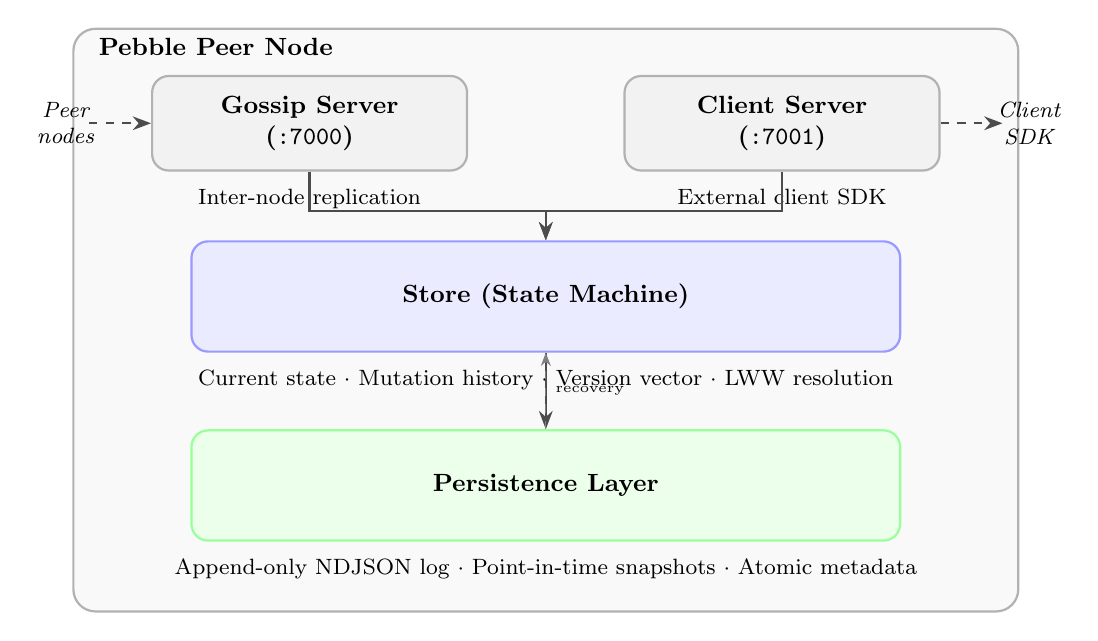
\begin{tikzpicture}[font=\small]

  % Outer node box
  \draw[draw=gray!60, fill=gray!5, rounded corners=8pt, thick]
    (-0.5, -0.2) rectangle (11.5, 7.2);
  \node[anchor=north west, font=\bfseries\small] at (-0.3, 7.2)
    {Pebble Peer Node};

  % Gossip Server
  \node[component, minimum width=4cm, minimum height=1.2cm, align=center]
    (gossip) at (2.5, 6) {Gossip Server\\(\texttt{:7000})};
  \node[font=\footnotesize, below=0pt of gossip, yshift=-0.1cm]
    {Inter-node replication};

  % Client Server
  \node[component, minimum width=4cm, minimum height=1.2cm, align=center]
    (client) at (8.5, 6) {Client Server\\(\texttt{:7001})};
  \node[font=\footnotesize, below=0pt of client, yshift=-0.1cm]
    {External client SDK};

  % Store
  \node[component, minimum width=9cm, minimum height=1.4cm,
        fill=blue!8, draw=blue!40]
    (store) at (5.5, 3.8) {Store (State Machine)};
  \node[font=\footnotesize, below=0pt of store, yshift=-0.1cm]
    {Current state $\cdot$ Mutation history $\cdot$ Version vector $\cdot$ LWW resolution};

  % Persistence
  \node[component, minimum width=9cm, minimum height=1.4cm,
        fill=green!8, draw=green!40]
    (persist) at (5.5, 1.4) {Persistence Layer};
  \node[font=\footnotesize, below=0pt of persist, yshift=-0.1cm]
    {Append-only NDJSON log $\cdot$ Point-in-time snapshots $\cdot$ Atomic metadata};

  % Arrows
  \draw[msg arrow] (gossip.south) -- ++(0,-0.5) -| (store.north);
  \draw[msg arrow] (client.south) -- ++(0,-0.5) -| (store.north);
  \draw[msg arrow] (store.south) -- (persist.north);
  \draw[dashed arrow] (persist.north) -- node[right, font=\tiny]{recovery} (store.south);

  % External labels
  \node[font=\footnotesize\itshape, align=center, left=0.6cm of gossip] {Peer\\nodes};
  \draw[msg arrow, dashed] (-0.3, 6) -- (gossip.west);
  \node[font=\footnotesize\itshape, align=center, right=0.6cm of client] {Client\\SDK};
  \draw[msg arrow, dashed] (client.east) -- (11.3, 6);

\end{tikzpicture}
\caption{Internal architecture of a \pebble{} peer node.}
\label{fig:node-arch}
\end{figure}

\paragraph{Gossip Port (\texttt{:7000}).}
Dedicated exclusively to inter-node communication. All gossip sessions begin
with a 3-way challenge-response handshake (\cref{sec:nodeauth}) to mutually
authenticate the connecting peer. Once established, the connection carries
\msg{PING}/\msg{PONG} health probes and the 4-step symmetric synchronisation
protocol (\cref{sec:gossip}). External clients never access this port.

\paragraph{Client Port (\texttt{:7001}).}
Dedicated to the external \pkg{client} SDK. Each connection undergoes a
2-message credential challenge (\cref{sec:clientauth}) before any key-value
operations are processed. Peer nodes never use this port.

This strict separation simplifies permission enforcement, enables independent
scaling of client-facing and replication-facing capacity, and eliminates any
ambiguity about which authentication path applies to a given connection.

\subsection{Package Dependency Graph}

\pebble{} is factored into seven packages that form a strict layered dependency
graph with no cycles:

\begin{figure}[H]
\centering
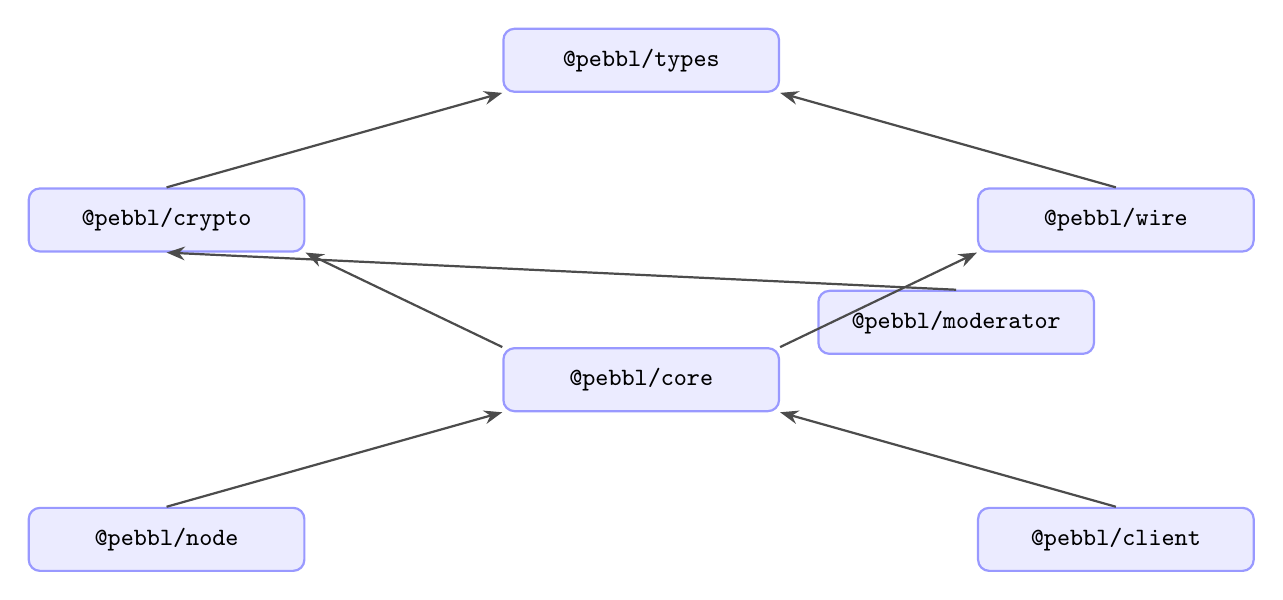
\begin{tikzpicture}[font=\small, node distance=1.2cm and 2.5cm]

  \node[node box, minimum width=3.5cm] (types)   {\pkg{types}};

  \node[node box, minimum width=3.5cm, below left=of types]
    (crypto) {\pkg{crypto}};
  \node[node box, minimum width=3.5cm, below right=of types]
    (wire)   {\pkg{wire}};

  \node[node box, minimum width=3.5cm, below right=of crypto]
    (core)   {\pkg{core}};

  \node[node box, minimum width=3.5cm, below left=of core]
    (node)   {\pkg{node}};
  \node[node box, minimum width=3.5cm, below right=of core]
    (clnt)   {\pkg{client}};

  \node[node box, minimum width=3.5cm, below=2.5cm of types, xshift=4cm]
    (mod)    {\pkg{moderator}};

  \draw[msg arrow] (crypto.north) -- (types.south west);
  \draw[msg arrow] (wire.north)   -- (types.south east);
  \draw[msg arrow] (core.north west) -- (crypto.south east);
  \draw[msg arrow] (core.north east) -- (wire.south west);
  \draw[msg arrow] (node.north) -- (core.south west);
  \draw[msg arrow] (clnt.north) -- (core.south east);
  \draw[msg arrow] (mod.north)  -- (crypto.south);

\end{tikzpicture}
\caption{Inter-package dependency graph. Arrows point from dependent to dependency.
\pkg{moderator} is an offline utility with no runtime dependency on \pkg{node}.}
\label{fig:dep-graph}
\end{figure}

\begin{table}[H]
\centering
\caption{Package responsibilities.}
\label{tab:packages}
\begin{tabular}{@{}lll@{}}
\toprule
\textbf{Package} & \textbf{Path} & \textbf{Responsibility} \\
\midrule
\pkg{types}     & \texttt{packages/types}     & Shared domain interfaces, protocol constants,
                                                 error classes. Zero dependencies. \\
\pkg{crypto}    & \texttt{packages/crypto}    & Ed25519 key generation, canonical JSON encoding,
                                                 mutation and credential signing. \\
\pkg{wire}      & \texttt{packages/wire}      & Length-type-payload TCP framing and stateful
                                                 stream decoder. \\
\pkg{core}      & \texttt{packages/core}      & In-memory Store, LWW conflict resolution,
                                                 append-only log, snapshots, crash recovery. \\
\pkg{node}      & \texttt{packages/node}      & Gossip engine, handshake, client server,
                                                 health monitoring, top-level orchestrator. \\
\pkg{client}    & \texttt{packages/client}    & Client SDK with multiplexed request tracking
                                                 and automatic authentication. \\
\pkg{moderator} & \texttt{packages/moderator} & Offline credential issuance and keypair
                                                 generation. \\
\bottomrule
\end{tabular}
\end{table}

\subsection{Data Flow Summary}

A write operation flows through the following components:

\begin{enumerate}[leftmargin=1.5em]
  \item \textbf{Client SDK} sends a \msg{PUT\_REQUEST} over the client port.
  \item \textbf{Client Server} verifies the client's session, enforces
        \texttt{read-write} permission, and forwards the request to the \textbf{Store}.
  \item \textbf{Store} creates an immutable signed mutation, applies LWW
        resolution, and emits a \texttt{mutation:applied} event.
  \item \textbf{Pebble (orchestrator)} listens to the event and appends the
        mutation to the \textbf{Mutation Log} with \texttt{fsync}.
  \item \textbf{Gossip Engine} periodically connects to healthy peers and
        transfers mutations they have not yet seen, as determined by comparing
        version vectors.
\end{enumerate}

% =============================================================================
% Section 3 — Data Model & Mutation Algebra
% =============================================================================
\section{Data Model and Mutation Algebra}
\label{sec:datamodel}

\subsection{The Mutation}

The fundamental unit of state change in \pebble{} is the \emph{mutation}---an
immutable, signed record of a single key-value operation.

\begin{definition}[Mutation]
\label{def:mutation}
A \emph{mutation} is a 7-tuple
\[
  m = \langle \mnid,\; \mseq,\; \mts,\; \mop,\; \mkey,\; \mval,\; \msig \rangle
\]
where:
\begin{itemize}[leftmargin=1.5em]
  \item $\mnid \in \NodeSet$ is the identifier of the node that created $m$.
  \item $\mseq \in \mathbb{Z}^{+}$ is a monotonically increasing counter local
        to $\mnid$: no two mutations from the same node share the same sequence
        number, and sequence numbers only increase across node restarts.
  \item $\mts \in \mathbb{Z}^{+}$ is the wall-clock timestamp (milliseconds
        since the Unix epoch) at the time of creation.
  \item $\mop \in \{\texttt{put},\; \texttt{delete}\}$ is the operation type.
  \item $\mkey \in \KeySet$ is the key being modified.
  \item $\mval \in \Sigma^* \cup \{\bot\}$ is the value: a non-empty UTF-8
        string for \texttt{put}, and $\bot$ (null) for \texttt{delete}.
  \item $\msig \in \{0,1\}^{512}$ is the Ed25519 signature of the node over
        all other fields (see \cref{sec:crypto}).
\end{itemize}
\end{definition}

\begin{definition}[Mutation ID]
\label{def:mutid}
The \emph{mutation ID} of $m$ is the pair $(\mnid, \mseq)$, written
$\mathrm{id}(m) = \mnid\texttt{:}\mseq$.
Mutation IDs are globally unique across the cluster:
\[
  \forall m, m' \in \MutSet:\quad
  \mathrm{id}(m) = \mathrm{id}(m') \implies m = m'.
\]
This is enforced by the sequence collision check in the Store
(see \cref{sec:invariants}, Invariant~\ref{inv:uniqueness}).
\end{definition}

\subsection{Operations and Tombstones}

\pebble{} supports exactly two operations:

\begin{description}[leftmargin=1.5em]
  \item[\texttt{put}$(k, v)$] Associates key $k$ with value $v \in \Sigma^*$.
  \item[\texttt{delete}$(k)$] Creates a \emph{tombstone} mutation for key $k$
        with $\mval = \bot$. The tombstone propagates through gossip like any
        other mutation, preventing deleted data from reappearing on nodes that
        have not yet received the deletion.
\end{description}

\begin{definition}[Live key]
A key $k$ is \emph{live} at node $n$ at time $t$ if the winning mutation for $k$
in $n$'s store has operation \texttt{put}. A key is \emph{deleted} if the winner
is a tombstone. A key is \emph{absent} if no mutation for $k$ has been received.
\end{definition}

\begin{remark}[Tombstone replication]
Tombstones must replicate through gossip exactly like writes. Without tombstone
replication, a node that has received a \texttt{put} but not yet received the
subsequent \texttt{delete} will continue to serve the stale value indefinitely.
\pebble{} stores tombstones in the mutation history and transfers them during
gossip sync. Tombstone GC is a v0.2 concern (\cref{sec:limitations}).
\end{remark}

\subsection{The Mutation History}

Every \pebble{} node maintains an in-memory \emph{mutation history}---a mapping
from mutation IDs to the corresponding full mutation objects:

\[
  H : (\NodeSet \times \mathbb{Z}^{+}) \to \MutSet
\]

The history grows monotonically: once a mutation is added it is never removed
(v0.1). The history enables exact range-based gossip: given a peer's version
vector, the local node can enumerate precisely which mutations the peer is missing.

\subsection{Current State}

The \emph{current state} is the projection of the history onto the winning
mutation per key:

\[
  S : \KeySet \to \MutSet,\quad S(k) = \win\bigl(\{m \in H : m.\mkey = k\}\bigr)
\]

where $\win$ is defined by the LWW total order of \cref{sec:conflict}.
The current state is maintained incrementally: when a new mutation $m$ for key
$k$ arrives, $S(k)$ is updated only if $m$ wins over the existing $S(k)$.

\subsection{Mutation Wire Format}

Mutations are serialised as JSON objects when transmitted over the gossip
protocol or stored in the mutation log. The canonical on-wire representation is:

\begin{lstlisting}[language=json, caption={Mutation JSON representation.}]
{
  "nodeId":    "node-a",
  "sequence":  42,
  "timestamp": 1787060000000,
  "operation": "put",
  "key":       "app:theme",
  "value":     "dark",
  "signature": "3045022100..."
}
\end{lstlisting}

\noindent For \texttt{delete} mutations, \texttt{"value"} is \texttt{null}.
The \texttt{signature} field covers all other fields via the canonical JSON
encoding described in \cref{sec:crypto}.

% =============================================================================
% Section 4 — Cryptographic Layer
% =============================================================================
\section{Cryptographic Layer}
\label{sec:crypto}

\pebble{} uses Ed25519~\cite{bernstein2012ed25519,rfc8032} for all digital
signatures. Ed25519 offers 128-bit security, fast verification, small 64-byte
signatures, and no per-signature randomness requirement, making it well-suited
for a high-throughput distributed system.

\subsection{Node Identity and Key Derivation}

Each node possesses a unique cryptographic identity generated once and persisted
to \texttt{\{dataDir\}/identity.json}.

\begin{definition}[Node identity]
A node's identity is a triple $\mathcal{I} = (\mathrm{nodeId},\, pk,\, sk)$
where:
\begin{itemize}[leftmargin=1.5em]
  \item $(pk, sk)$ is an Ed25519 key pair. $pk \in \{0,1\}^{256}$,
        $sk \in \{0,1\}^{256}$ (the seed).
  \item $\mathrm{nodeId} = \mathrm{base64url}\bigl(\mathrm{SHA\text{-}256}(pk)\bigr)$
        is the globally unique node identifier, derived deterministically from the
        public key.
\end{itemize}
\end{definition}

The identity file is created on first start and loaded on subsequent starts,
ensuring the same \texttt{nodeId} across restarts. The private key seed is
stored in hex encoding and never transmitted over any network interface.

\subsection{Canonical JSON Serialisation}

To produce a deterministic byte sequence for signing, \pebble{} implements a
canonical JSON encoder inspired by RFC~8785~\cite{rfc8785}.

\begin{definition}[Canonical encoding]
\label{def:canonical}
$\mathrm{canonicalEncode}(v)$ serialises a JSON-compatible value $v$ to a
UTF-8 byte string such that:
\begin{enumerate}[leftmargin=1.5em]
  \item Object keys are sorted lexicographically by their UTF-16 code units
        (matching the ECMAScript \texttt{localeCompare} order).
  \item No insignificant whitespace is emitted.
  \item Numbers are represented in their shortest round-trip form.
  \item String escaping follows JSON specification.
\end{enumerate}
\end{definition}

The canonical encoder is the only source of truth for the byte sequence
presented to the signing primitive. Any serialisation discrepancy would cause
valid signatures to appear invalid; therefore the encoder is tested with a
deterministic golden-value test suite.

\subsection{Mutation Signing and Verification}

\begin{definition}[Signable mutation fields]
The \emph{signable fields} of a mutation $m$ are all fields except $\msig$
itself:
\[
  m_{\text{sign}} =
    \langle m.\mnid,\; m.\mseq,\; m.\mts,\; m.\mop,\; m.\mkey,\; m.\mval \rangle
\]
\end{definition}

\begin{protocol}[Mutation signing]
To create a signed mutation at node $n$ with identity $\mathcal{I}_n$:
\begin{enumerate}[leftmargin=1.5em]
  \item Assemble $m_{\text{sign}}$ with all fields populated.
  \item Compute $b = \mathrm{canonicalEncode}(m_{\text{sign}})$.
  \item Compute $\msig = \mathrm{Ed25519Sign}(sk_n,\, b)$.
  \item Return $m = m_{\text{sign}} \cup \{\msig\}$.
\end{enumerate}
\end{protocol}

\begin{protocol}[Mutation verification]
\label{proto:verify-mut}
To verify a mutation $m$ received from a peer, given the originating node's
public key $pk_{\mnid}$ obtained from the cluster configuration:
\begin{enumerate}[leftmargin=1.5em]
  \item Extract $m_{\text{sign}} = m \setminus \{\msig\}$.
  \item Compute $b = \mathrm{canonicalEncode}(m_{\text{sign}})$.
  \item Return $\mathrm{Ed25519Verify}(pk_{\mnid},\, b,\, m.\msig)$.
\end{enumerate}
If the originating \texttt{nodeId} is not present in the cluster configuration,
verification fails with an \texttt{UnknownNodeError} before the signature is
even checked.
\end{protocol}

\begin{remark}[Startup recovery bypass]
During crash recovery (\cref{sec:persistence}), mutations are replayed from the
local on-disk log with signature verification \emph{skipped}. This is safe
because:
(1)~the log is written by the local node and protected by OS file permissions;
(2)~any mutation in the log was either created locally (and therefore valid) or
received from a peer and verified at application time before being persisted.
The \texttt{skipSignatureVerification} flag is never set for mutations received
over the network.
\end{remark}

\subsection{Moderator Credential System}

External client access is controlled through a lightweight certificate-authority
(CA) model. The \emph{moderator} is an offline entity that holds the cluster's
root signing key.

\begin{definition}[Client credential]
\label{def:credential}
A \emph{client credential} is a 6-tuple signed by the moderator:
\[
  C = \langle \mathit{clientId},\; pk_c,\; \mathit{perm},\;
              t_{\text{issued}},\; t_{\text{expires}},\; \msig_{\text{mod}} \rangle
\]
where:
\begin{itemize}[leftmargin=1.5em]
  \item $\mathit{clientId}$ is a human-readable client identifier.
  \item $pk_c \in \{0,1\}^{256}$ is the client's Ed25519 public key.
  \item $\mathit{perm} \in \{\texttt{read-only},\; \texttt{read-write}\}$ is
        the access level granted.
  \item $t_{\text{issued}},\; t_{\text{expires}} \in \mathbb{Z}$ are Unix
        millisecond timestamps ($t_{\text{expires}} = \bot$ for no expiry).
  \item $\msig_{\text{mod}} = \mathrm{Ed25519Sign}\bigl(sk_{\text{mod}},\;
        \mathrm{canonicalEncode}(\langle\mathit{clientId}, pk_c, \mathit{perm},
        t_{\text{issued}}, t_{\text{expires}}\rangle)\bigr)$.
\end{itemize}
\end{definition}

Credential issuance is performed offline using \pkg{moderator} and does not
require modifying \texttt{cluster.json} or restarting running nodes. The
moderator's public key $pk_{\text{mod}}$ is stored in the cluster configuration
and used by every node to verify incoming credentials.

\begin{remark}[Security properties]
The credential system provides:
\begin{itemize}[leftmargin=1.5em]
  \item \textbf{Unforgeability}: only the holder of $sk_{\text{mod}}$ can issue
        valid credentials.
  \item \textbf{Expiry enforcement}: nodes reject credentials where
        $\mathrm{now}() > t_{\text{expires}}$.
  \item \textbf{Key binding}: during the AUTH handshake, the client proves
        possession of $sk_c$ by signing a fresh nonce, preventing credential
        replay from a different identity.
\end{itemize}
\end{remark}

% =============================================================================
% Section 5 — Conflict Resolution (LWW)
% =============================================================================
\section{Conflict Resolution: Deterministic Last-Write-Wins}
\label{sec:conflict}

When two mutations target the same key and arrive at a node in different orders
on different peers, the nodes must converge to the same winner without
coordination. \pebble{} achieves this through a deterministic total order on
mutations---Last-Write-Wins (LWW).

\subsection{The LWW Total Order}

\begin{definition}[LWW comparison]
\label{def:lww-order}
Define the relation $\lwwlt$ on mutations $a, b \in \MutSet$ as follows:
\[
  a \lwwlt b \;\iff\;
  \begin{cases}
    a.\mts < b.\mts, & \\
    \text{or}\quad a.\mts = b.\mts \;\land\; a.\mnid <_{\mathrm{lex}} b.\mnid, & \\
    \text{or}\quad a.\mts = b.\mts \;\land\; a.\mnid = b.\mnid
               \;\land\; a.\mseq < b.\mseq. &
  \end{cases}
\]
\end{definition}

In prose: the mutation with the \emph{higher timestamp} wins. Ties are broken by
the \emph{lexicographically later node ID}; this is arbitrary but stable across
all nodes because every node applies the same comparison function. A further
tiebreak on \emph{higher sequence} handles the degenerate case of two mutations
from the same node with the same timestamp (possible under fast local writes).

\begin{definition}[Winner]
\label{def:winner}
Given two mutations $a$ and $b$ for the same key, the winner is:
\[
  \win(a, b) =
  \begin{cases}
    b & \text{if } a \lwwlt b, \\
    a & \text{otherwise.}
  \end{cases}
\]
\end{definition}

\subsection{Proof: $\lwwlt$ is a Strict Total Order}

\begin{theorem}[$\lwwlt$ is a strict total order on $\MutSet$]
\label{thm:total-order}
The relation $\lwwlt$ is irreflexive, asymmetric, transitive, and total on
the set of all mutations $\MutSet$.
\end{theorem}

\begin{proof}
We verify each property:

\paragraph{Irreflexivity.}
$a \lwwlt a$ would require $a.\mts < a.\mts$ (false), or $a.\mts = a.\mts$ and
$a.\mnid <_{\mathrm{lex}} a.\mnid$ (false), or all equal and $a.\mseq < a.\mseq$
(false). Hence $a \not\lwwlt a$. \checkmark

\paragraph{Asymmetry (implies antisymmetry).}
Suppose $a \lwwlt b$. We show $b \not\lwwlt a$.
If $a \lwwlt b$ holds because $a.\mts < b.\mts$, then $b.\mts > a.\mts$,
so the first clause of $b \lwwlt a$ is false. The remaining clauses require
$b.\mts = a.\mts$, which is also false. Hence $b \not\lwwlt a$.
The remaining two cases proceed analogously by the asymmetry of $<$ and
$<_{\mathrm{lex}}$. \checkmark

\paragraph{Transitivity.}
Suppose $a \lwwlt b$ and $b \lwwlt c$. We show $a \lwwlt c$ by case analysis
on which clause governs each relation:
\begin{itemize}[leftmargin=1.5em]
  \item If $a.\mts < b.\mts$ and $b.\mts \leq c.\mts$, then $a.\mts < c.\mts$,
        so the first clause of $a \lwwlt c$ holds.
  \item If $a.\mts = b.\mts$ and $b.\mts = c.\mts$ (i.e., all equal), then
        the governing clause is on $\mnid$ or $\mseq$, both of which are
        transitively ordered by the transitivity of $<_{\mathrm{lex}}$ and $<$.
  \item Mixed cases (e.g., $a.\mts < b.\mts$ and $b.\mts = c.\mts$) collapse
        to $a.\mts < c.\mts$ by substitution. \checkmark
\end{itemize}

\paragraph{Totality.}
For any $a \neq b$, either $a.\mts \neq b.\mts$ (handled by the first clause),
or $a.\mnid \neq b.\mnid$ (handled by the second, since $<_{\mathrm{lex}}$ is
total on strings), or $a.\mseq \neq b.\mseq$ (handled by the third, since $<$
is total on integers). The only remaining case is $a = b$, which is excluded.
Hence exactly one of $a \lwwlt b$ or $b \lwwlt a$ holds for $a \neq b$. \checkmark
\end{proof}

\subsection{Convergence Theorem}

\begin{theorem}[Convergence under LWW]
\label{thm:convergence}
Let $n_1, n_2$ be two nodes that have received (in any order) the same set of
mutations $M$ for a key $k$. Both nodes independently compute the same current
value for $k$.
\end{theorem}

\begin{proof}
By \cref{thm:total-order}, $\lwwlt$ is a strict total order on $\MutSet$.
Therefore, the set $\{m \in M : m.\mkey = k\}$ has a unique maximum element
$m^*$ under $\lwwlt$. The function $\win$ selects this maximum deterministically.
Because $\win$ is a function solely of the mutation set---not of arrival
order---both nodes compute the same $m^*$ regardless of the order in which
they processed mutations from $M$. \qed
\end{proof}

\begin{corollary}[Eventual consistency]
\label{cor:eventual}
If the gossip protocol ensures that every mutation created at any node is
eventually delivered to every other node (i.e., the network is eventually
connected), then all nodes eventually agree on the value of every key.
\end{corollary}

\subsection{Implementation}

The comparison function is implemented in \texttt{packages/core/src/store/conflict.ts}:

\begin{lstlisting}[caption={LWW comparison function (TypeScript).}]
export function compare(a: Mutation, b: Mutation): number {
  if (a.timestamp !== b.timestamp) return a.timestamp - b.timestamp;
  if (a.nodeId   !== b.nodeId)   return a.nodeId.localeCompare(b.nodeId);
  return a.sequence - b.sequence;
}

export function winner(incumbent: Mutation, challenger: Mutation): Mutation {
  return compare(challenger, incumbent) > 0 ? challenger : incumbent;
}
\end{lstlisting}

A positive return value indicates the challenger wins; the Store updates
\texttt{currentState[key]} only when the incoming mutation defeats the incumbent.

\subsection{Clock Skew Limitation}

The LWW order as defined relies on wall-clock timestamps. A node whose clock
runs significantly behind can produce mutations that lose to older writes on
other nodes, even if the losing mutation was authored later in real time.
\pebble{} v0.1 accepts this trade-off for simplicity. \Cref{sec:future}
discusses Hybrid Logical Clocks (HLC)~\cite{kulkarni2014hlc} as a path to
causality-aware conflict resolution.

% =============================================================================
% Section 6 — Version Vectors
% =============================================================================
\section{Version Vectors and Incremental Synchronisation}
\label{sec:vv}

Version vectors~\cite{fidge1988timestamps,mattern1989vector} are the mechanism
by which \pebble{} nodes summarise their mutation history and compute precisely
which mutations a peer is missing, without enumerating the entire history.

\subsection{Definition}

\begin{definition}[Version vector]
\label{def:vv}
A \emph{version vector} is a partial function
\[
  V : \NodeSet \rightharpoonup \mathbb{Z}^{+}
\]
mapping each known node identifier to the \emph{highest sequence number} seen
from that node. Entries absent from $V$ are treated as $0$:
$V[n] \triangleq 0$ if $n \notin \mathrm{dom}(V)$.
\end{definition}

\begin{remark}[High-water mark semantics]
\pebble{} v0.1 uses a \emph{contiguous high-water mark}: $V[n] = s$ implies
that this node has received \emph{all} of node $n$'s mutations with sequence
$1, 2, \ldots, s$. This assumption is valid because:
\begin{enumerate}[leftmargin=1.5em]
  \item Mutations from the same originating node are applied in the gossip
        response in sequence order.
  \item A single TCP connection is used per gossip session; TCP guarantees
        in-order delivery within the session.
\end{enumerate}
\cref{sec:limitations} discusses the implications of this assumption for
out-of-order delivery.
\end{remark}

\subsection{Vector Advancement}

When a mutation $m$ is applied to the store, the local version vector is advanced:

\begin{definition}[Vector advancement]
\[
  \mathrm{advance}(V, m) : \quad V[m.\mnid] \;\leftarrow\; \max\bigl(V[m.\mnid],\; m.\mseq\bigr)
\]
\end{definition}

The use of $\max$ ensures the vector is \emph{monotonically non-decreasing}: once
a sequence number is recorded for a node, it is never reduced. This satisfies
Invariant~\ref{inv:mono-vec} (\cref{sec:invariants}).

\subsection{Missing-Range Computation}

The core of incremental gossip synchronisation is computing which mutations one
node needs from another.

\begin{definition}[Missing ranges]
\label{def:missing-ranges}
Given the local node's vector $V_A$ and the peer's vector $V_B$, the ranges
that the peer is missing (i.e., mutations the local node has but the peer does not)
are:
\[
  \mathrm{missing}(V_A, V_B) \;=\;
  \bigl\{\; (n,\; V_B[n]+1,\; V_A[n])
  \;\mutid\; n \in \mathrm{dom}(V_A) \;\land\; V_A[n] > V_B[n] \;\bigr\}
\]
Each element $(n, \mathit{from}, \mathit{to})$ represents the sequence range
$[\mathit{from}, \mathit{to}]$ for node $n$.
\end{definition}

\begin{example}
Suppose $V_A = \{n_1 \mapsto 5,\; n_2 \mapsto 3\}$ and
$V_B = \{n_1 \mapsto 3,\; n_3 \mapsto 2\}$.

Then:
\[
  \mathrm{missing}(V_A, V_B) = \{(n_1, 4, 5),\; (n_2, 1, 3)\}
\]
Node $B$ is missing mutations $4$ and $5$ from $n_1$, and all mutations $1$--$3$
from $n_2$. Note: $n_3$ entries in $V_B$ that are absent from $V_A$ are irrelevant
to what $A$ can send $B$.
\end{example}

\begin{remark}[Symmetric computation]
In a gossip round, both nodes compute missing ranges for the other:
\begin{itemize}[leftmargin=1.5em]
  \item $A$ computes $\mathrm{missing}(V_B, V_A)$ --- what $A$ needs from $B$.
  \item $B$ computes $\mathrm{missing}(V_A, V_B)$ --- what $B$ needs from $A$.
\end{itemize}
After exchanging DIGESTs, each node has both vectors and can compute its own
request set, enabling the symmetric 4-step protocol of \cref{sec:gossip}.
\end{remark}

\subsection{Monotonicity Invariant}

\begin{invariant}[Monotonic version vectors]
\label{inv:mono-vv}
For any node $n$ and any node identifier $n'$, $V_n[n']$ is non-decreasing
over time. Formally, if event $e_1$ happens-before event $e_2$ at node $n$,
then $V_n^{e_1}[n'] \leq V_n^{e_2}[n']$.
\end{invariant}

\begin{proof}
The advancement operation uses $\max$, which is monotonically non-decreasing.
Vector entries are only ever written through $\mathrm{advance}$, and no code
path decreases a vector entry. \qed
\end{proof}

\subsection{Protocol Limits on Ranges}

To prevent a single gossip message from becoming arbitrarily large, \pebble{}
caps the number of requested ranges per message at
\texttt{limits.maxRangesPerRequest} (default: 100) and the number of mutations
per MUTATIONS message at \texttt{limits.maxMutationsPerMessage} (default: 500).
A node that is severely behind will catch up over multiple gossip rounds.

% =============================================================================
% Section 7 — Gossip Protocol
% =============================================================================
\section{Gossip Protocol: 4-Step Symmetric Synchronisation}
\label{sec:gossip}

\pebble{} uses a \emph{pull-based, symmetric gossip protocol}~\cite{demers1987epidemic,
kermarrec2007gossip} for replication. Every \texttt{gossipIntervalMs} milliseconds,
each node selects one healthy peer (random selection among healthy nodes) and
runs a complete sync session with it.

\subsection{Session Overview}

Each gossip session consists of exactly four steps, alternating message ownership
between the initiator and responder. Both sides make progress in each round.

\begin{figure}[H]
\centering
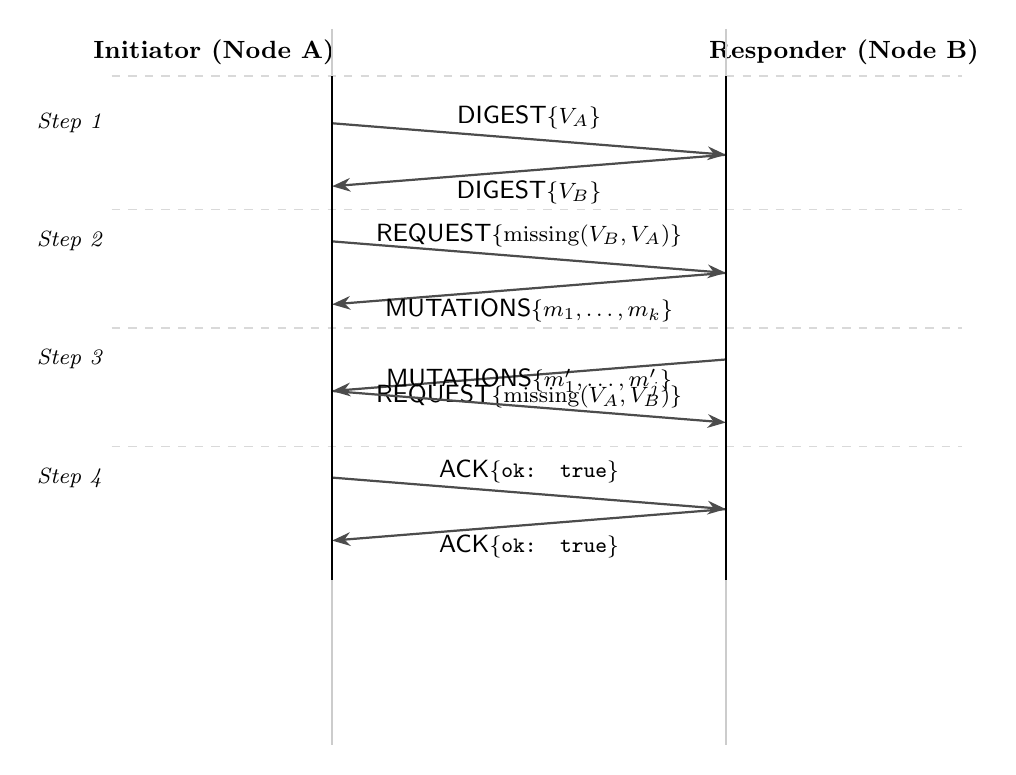
\begin{tikzpicture}[font=\small, node distance=0.1cm]

  % Column headers
  \node (A) at (1.5, 8.5) {\textbf{Initiator (Node A)}};
  \node (B) at (9.5, 8.5) {\textbf{Responder (Node B)}};
  \draw[thick, gray!40] (3, 8.8) -- (3, -0.3);
  \draw[thick, gray!40] (8, 8.8) -- (8, -0.3);
  \draw[dashed, gray!30] (0.2, 8.2) -- (11, 8.2);

  % Step 1 label
  \node[font=\footnotesize\itshape, left] at (0.2, 7.6) {Step 1};

  % DIGEST A -> B
  \draw[msg arrow] (3, 7.6) -- (8, 7.2)
    node[midway, above, font=\footnotesize]
    {\msg{DIGEST}\{$V_A$\}};
  % DIGEST B -> A
  \draw[msg arrow] (8, 7.2) -- (3, 6.8)
    node[midway, below, font=\footnotesize]
    {\msg{DIGEST}\{$V_B$\}};

  \draw[dashed, gray!30] (0.2, 6.5) -- (11, 6.5);
  \node[font=\footnotesize\itshape, left] at (0.2, 6.1) {Step 2};

  % REQUEST A -> B
  \draw[msg arrow] (3, 6.1) -- (8, 5.7)
    node[midway, above, font=\footnotesize]
    {\msg{REQUEST}\{$\mathrm{missing}(V_B, V_A)$\}};
  % MUTATIONS B -> A
  \draw[msg arrow] (8, 5.7) -- (3, 5.3)
    node[midway, below, font=\footnotesize]
    {\msg{MUTATIONS}\{$m_1, \ldots, m_k$\}};

  \draw[dashed, gray!30] (0.2, 5.0) -- (11, 5.0);
  \node[font=\footnotesize\itshape, left] at (0.2, 4.6) {Step 3};

  % REQUEST B -> A
  \draw[msg arrow] (8, 4.6) -- (3, 4.2)
    node[midway, below, font=\footnotesize]
    {\msg{REQUEST}\{$\mathrm{missing}(V_A, V_B)$\}};
  % MUTATIONS A -> B
  \draw[msg arrow] (3, 4.2) -- (8, 3.8)
    node[midway, above, font=\footnotesize]
    {\msg{MUTATIONS}\{$m_1', \ldots, m_j'$\}};

  \draw[dashed, gray!30] (0.2, 3.5) -- (11, 3.5);
  \node[font=\footnotesize\itshape, left] at (0.2, 3.1) {Step 4};

  % ACK A -> B
  \draw[msg arrow] (3, 3.1) -- (8, 2.7)
    node[midway, above, font=\footnotesize]
    {\msg{ACK}\{\texttt{ok: true}\}};
  % ACK B -> A
  \draw[msg arrow] (8, 2.7) -- (3, 2.3)
    node[midway, below, font=\footnotesize]
    {\msg{ACK}\{\texttt{ok: true}\}};

  % Lifecycle lines
  \draw[thick] (3, 8.2) -- (3, 1.8);
  \draw[thick] (8, 8.2) -- (8, 1.8);

\end{tikzpicture}
\caption{4-step symmetric gossip protocol. After exchanging DIGESTs, each side
requests and receives the mutations it is missing.}
\label{fig:gossip-protocol}
\end{figure}

\subsection{Step-by-Step Description}

\paragraph{Step 1 — DIGEST exchange.}
Both nodes send their current version vectors simultaneously. After this step,
each node holds both $V_A$ and $V_B$ and can independently compute the ranges
that the other is missing.

\paragraph{Step 2 — Initiator requests and receives.}
The initiator computes $\mathrm{missing}(V_B, V_A)$ (what $A$ needs from $B$)
and sends a \msg{REQUEST} message. The responder looks up the requested
mutations in its history and sends them in a \msg{MUTATIONS} message. The
initiator applies each received mutation through the store's
\texttt{applyMutation} pipeline (including signature verification).

\paragraph{Step 3 — Responder requests and receives.}
The responder computes $\mathrm{missing}(V_A, V_B)$ (what $B$ needs from $A$)
and sends a \msg{REQUEST}. The initiator replies with the matching mutations.

\paragraph{Step 4 — ACK.}
Both sides send \msg{ACK} to signal successful completion. The gossip engine
records a successful round and updates the peer's health state.

\subsection{Protocol Properties}

\begin{theorem}[Deadlock freedom]
\label{thm:deadlock-free}
The 4-step gossip protocol is deadlock-free.
\end{theorem}

\begin{proof}
The message sequence is fixed and deterministic: initiator sends, then
responder sends, alternating for exactly 4 sub-steps. Neither side waits for
the other to initiate a send before completing its own step. Each
\texttt{send}/\texttt{receive} call on a connection is backed by a buffered
TCP socket; a send never blocks waiting for the remote side to call \texttt{receive}
on the same message. Since the turn sequence is fixed and finite, no circular
waiting condition can arise. \qed
\end{proof}

\begin{theorem}[Idempotency]
\label{thm:idempotent}
Applying a mutation that has already been applied is a no-op.
\end{theorem}

\begin{proof}
Before applying any mutation $m$, \texttt{applyMutation} checks whether
$\mathrm{id}(m)$ already exists in the history map $H$. If it does, and the
stored content is byte-for-byte identical, the function returns \texttt{false}
without modifying state. If the stored content differs (a sequence collision),
an error is thrown (see Invariant~\ref{inv:uniqueness}). In the normal case,
duplicate mutations are silently dropped, making gossip delivery idempotent. \qed
\end{proof}

\subsection{Gossip Target Selection}

In each round, the \texttt{GossipEngine} calls
\texttt{PeerHealth.selectGossipTarget()}, which returns a random healthy peer
or \texttt{null} if none are available. This provides a simple, unbiased
gossip fanout of 1 per interval. The expected number of rounds for a mutation
to reach all $N$ nodes is $\Oof{N \log N}$ (see \cref{sec:complexity}).

\subsection{Health Monitoring}

The \texttt{Pinger} sends \msg{PING} messages to all peers every
\texttt{pingIntervalMs} milliseconds (default: 2,000\,ms) on the gossip port.
A peer is marked \emph{unhealthy} if no successful communication has been
observed in the past \texttt{unhealthyThresholdMs} milliseconds (default:
10,000\,ms). Unhealthy peers are excluded from gossip target selection but
remain in the configuration; they are automatically restored to healthy status
upon the next successful handshake.

% =============================================================================
% Section 8 — Node Authentication (3-Way Handshake)
% =============================================================================
\section{Node Authentication: 3-Way Handshake}
\label{sec:nodeauth}

Before any gossip data exchange, two \pebble{} nodes perform a mutual
challenge-response handshake to authenticate each other and bind the connection
to the correct cluster. This prevents rogue nodes from injecting mutations into
a cluster and prevents cross-cluster contamination.

\subsection{Handshake Protocol}

\begin{figure}[H]
\centering
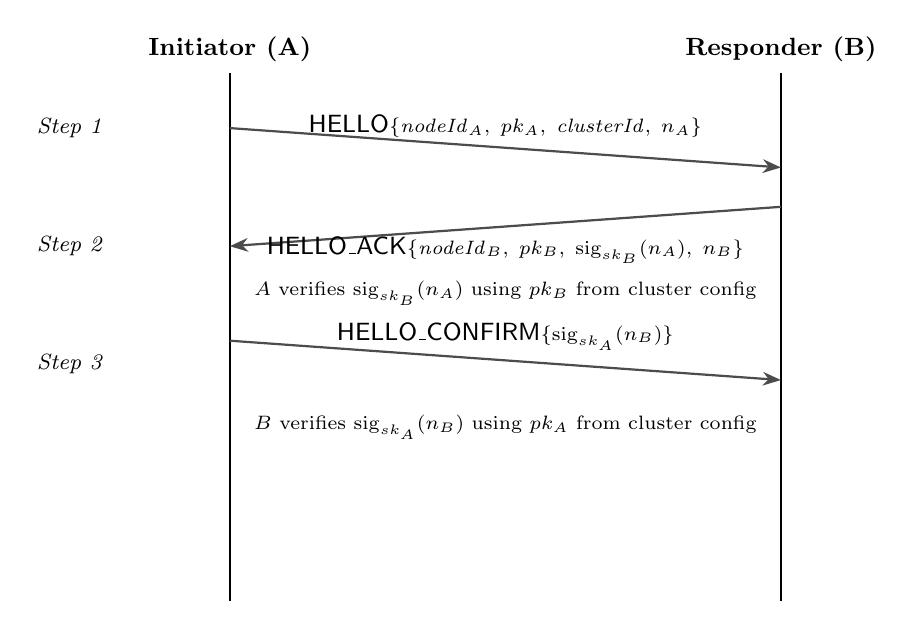
\begin{tikzpicture}[font=\small]

  % Headers
  \node at (2, 7.5) {\textbf{Initiator (A)}};
  \node at (9, 7.5) {\textbf{Responder (B)}};
  \draw[thick] (2, 7.2) -- (2, 0.5);
  \draw[thick] (9, 7.2) -- (9, 0.5);

  % Step 1: HELLO
  \node[font=\footnotesize\itshape, left] at (0.5, 6.5) {Step 1};
  \draw[msg arrow] (2, 6.5) -- (9, 6.0)
    node[midway, above, font=\scriptsize]
    {\msg{HELLO}\{$\mathit{nodeId}_A,\; pk_A,\; \mathit{clusterId},\; n_A$\}};

  % Step 2: HELLO_ACK
  \node[font=\footnotesize\itshape, left] at (0.5, 5.0) {Step 2};
  \draw[msg arrow] (9, 5.5) -- (2, 5.0)
    node[midway, below, font=\scriptsize]
    {\msg{HELLO\_ACK}\{$\mathit{nodeId}_B,\; pk_B,\; \mathrm{sig}_{sk_B}(n_A),\; n_B$\}};

  % Verify nonce_A_sig annotation
  \node[font=\scriptsize, align=left] at (5.5, 4.4)
    {$A$ verifies $\mathrm{sig}_{sk_B}(n_A)$ using $pk_B$ from cluster config};

  % Step 3: HELLO_CONFIRM
  \node[font=\footnotesize\itshape, left] at (0.5, 3.5) {Step 3};
  \draw[msg arrow] (2, 3.8) -- (9, 3.3)
    node[midway, above, font=\scriptsize]
    {\msg{HELLO\_CONFIRM}\{$\mathrm{sig}_{sk_A}(n_B)$\}};

  % Verify nonce_B_sig annotation
  \node[font=\scriptsize, align=left] at (5.5, 2.7)
    {$B$ verifies $\mathrm{sig}_{sk_A}(n_B)$ using $pk_A$ from cluster config};


\end{tikzpicture}
\caption{3-way mutual authentication handshake between peer nodes.
$n_A, n_B$ are fresh 128-bit nonces; $\mathrm{sig}_{sk}(x)$ denotes an
Ed25519 signature of $x$ under private key $sk$.}
\label{fig:handshake}
\end{figure}

\subsection{Step-by-Step Description}

\paragraph{Step 1 — HELLO.}
The initiator sends its node identity and a fresh 128-bit random nonce $n_A$:
\[
  A \to B:\; \msg{HELLO}\bigl\{\mnid_A,\; pk_A,\; \mathit{clusterId},\;
             \mathrm{version},\; n_A\bigr\}
\]
The cluster ID and protocol version are included so $B$ can reject connections
from different clusters or incompatible protocol versions immediately.

\paragraph{Step 2 — HELLO\_ACK.}
The responder validates:
\begin{enumerate}[leftmargin=1.5em]
  \item $\mathit{clusterId}$ matches its own configuration.
  \item $\mathrm{version} = 1$ (current protocol version).
  \item $\mnid_A$ is present in the cluster configuration and $pk_A$ matches.
\end{enumerate}
If any check fails, $B$ sends an \msg{ERROR} and closes the connection.
Otherwise, $B$ generates its own nonce $n_B$, signs $n_A$ with its private key,
and replies:
\[
  B \to A:\; \msg{HELLO\_ACK}\bigl\{\mnid_B,\; pk_B,\; \mathit{clusterId},\;
             \mathrm{sig}_{sk_B}(n_A),\; n_B\bigr\}
\]
$A$ then verifies that $\mnid_B$ is in its cluster configuration, that $pk_B$
matches, and that $\mathrm{sig}_{sk_B}(n_A)$ is a valid Ed25519 signature.

\paragraph{Step 3 — HELLO\_CONFIRM.}
The initiator signs $n_B$ with its own private key and sends:
\[
  A \to B:\; \msg{HELLO\_CONFIRM}\bigl\{\mathrm{sig}_{sk_A}(n_B)\bigr\}
\]
$B$ verifies the signature. Both sides have now mutually verified each other's
identity. The connection proceeds to gossip sync.

\subsection{Security Properties}

\begin{theorem}[Mutual authentication]
\label{thm:mutual-auth}
After a successful handshake, each node has verified that the peer holds the
private key corresponding to the public key registered in the cluster
configuration for that node's ID.
\end{theorem}

\begin{proof}
$B$ verifies $\mathrm{sig}_{sk_A}(n_B)$ using $pk_A$ from its \emph{local}
cluster configuration---not from the HELLO message itself. A successful
verification proves $A$ possesses $sk_A$ such that
$\mathrm{Ed25519Verify}(pk_A, n_B, \mathrm{sig}_{sk_A}(n_B)) = \top$.
Symmetrically, $A$ verifies $B$'s signature using the configuration-bound
$pk_B$. \qed
\end{proof}

\begin{theorem}[Replay resistance]
\label{thm:replay}
A handshake transcript cannot be replayed by an adversary to establish a new
authenticated connection.
\end{theorem}

\begin{proof}
The nonces $n_A$ and $n_B$ are generated freshly for each connection attempt
using a cryptographically secure random number generator. The signatures cover
these nonces, so any replay of a captured transcript will fail verification
because the nonces in the new challenge will differ. \qed
\end{proof}

\begin{theorem}[Cluster binding]
\label{thm:cluster-binding}
A node from cluster $C_1$ cannot successfully complete a handshake with a node
configured for cluster $C_2 \neq C_1$.
\end{theorem}

\begin{proof}
The cluster ID is checked in Step 2 before any signature is issued. A mismatch
causes an immediate \msg{ERROR}. \qed
\end{proof}

% =============================================================================
% Section 9 — Client Authentication & Permission System
% =============================================================================
\section{Client Authentication and Permission System}
\label{sec:clientauth}

External clients connect to the client port (\texttt{:7001}) and must present a
moderator-issued credential before any key-value operations are processed.
Authentication is performed through a 3-message challenge-response sequence.

\subsection{Authentication Protocol}

\begin{figure}[H]
\centering
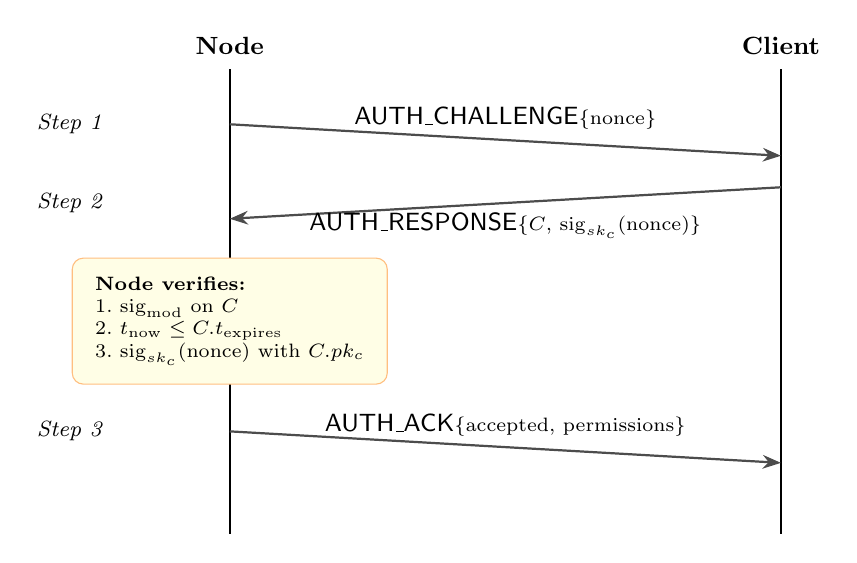
\begin{tikzpicture}[font=\small]

  \node at (2, 7.0) {\textbf{Node}};
  \node at (9, 7.0) {\textbf{Client}};
  \draw[thick] (2, 6.7) -- (2, 0.8);
  \draw[thick] (9, 6.7) -- (9, 0.8);

  % Step 1
  \node[font=\footnotesize\itshape, left] at (0.5, 6.0) {Step 1};
  \draw[msg arrow] (2, 6.0) -- (9, 5.6)
    node[midway, above, font=\scriptsize]
    {\msg{AUTH\_CHALLENGE}\{nonce\}};

  % Step 2
  \node[font=\footnotesize\itshape, left] at (0.5, 5.0) {Step 2};
  \draw[msg arrow] (9, 5.2) -- (2, 4.8)
    node[midway, below, font=\scriptsize]
    {\msg{AUTH\_RESPONSE}\{$C$, $\mathrm{sig}_{sk_c}(\mathrm{nonce})$\}};

  % Verification block
  \node[draw, rounded corners=4pt, fill=yellow!10, draw=orange!50,
        minimum width=4cm, minimum height=1.6cm, font=\scriptsize, align=left]
    (verify) at (2, 3.5) {
      \textbf{Node verifies:}\\
      1.\ $\mathrm{sig}_{\mathrm{mod}}$ on $C$\\
      2.\ $t_{\mathrm{now}} \leq C.t_{\mathrm{expires}}$\\
      3.\ $\mathrm{sig}_{sk_c}(\mathrm{nonce})$ with $C.pk_c$
    };

  % Step 3
  \node[font=\footnotesize\itshape, left] at (0.5, 2.1) {Step 3};
  \draw[msg arrow] (2, 2.1) -- (9, 1.7)
    node[midway, above, font=\scriptsize]
    {\msg{AUTH\_ACK}\{accepted, permissions\}};

\end{tikzpicture}
\caption{Client authentication protocol. $C$ is the credential bundle; $sk_c$
is the client's private key; $\mathrm{sig}_{\mathrm{mod}}$ is the moderator's
signature embedded in $C$.}
\label{fig:client-auth}
\end{figure}

\subsection{Step-by-Step Description}

\paragraph{Step 1 — AUTH\_CHALLENGE.}
Upon connection, the node generates a fresh 128-bit nonce and sends it
immediately:
\[
  \mathrm{Node} \to \mathrm{Client}:\; \msg{AUTH\_CHALLENGE}\{\mathrm{nonce}\}
\]
The client has a configurable timeout to respond.

\paragraph{Step 2 — AUTH\_RESPONSE.}
The client sends its credential bundle $C$ (as defined in
\cref{def:credential}) and a signature of the nonce under its private key:
\[
  \mathrm{Client} \to \mathrm{Node}:\;
  \msg{AUTH\_RESPONSE}\bigl\{C,\; \mathrm{sig}_{sk_c}(\mathrm{nonce})\bigr\}
\]

\paragraph{Step 3 — Verification and AUTH\_ACK.}
The node performs three sequential checks:
\begin{enumerate}[leftmargin=1.5em]
  \item \textbf{Moderator signature.}
    $\mathrm{Ed25519Verify}(pk_{\mathrm{mod}},\; \mathrm{canonicalEncode}(C \setminus \{\msig_{\mathrm{mod}}\}),\; C.\msig_{\mathrm{mod}})$
    must hold, using $pk_{\mathrm{mod}}$ from the cluster configuration.

  \item \textbf{Credential expiry.}
    If $C.t_{\mathrm{expires}} \neq \bot$, then
    $\mathrm{now}() \leq C.t_{\mathrm{expires}}$ must hold.

  \item \textbf{Proof of key possession.}
    $\mathrm{Ed25519Verify}(C.pk_c,\; \mathrm{nonce},\; \mathrm{sig}_{sk_c}(\mathrm{nonce}))$
    must hold.
\end{enumerate}
If all checks pass, the node sends:
\[
  \mathrm{Node} \to \mathrm{Client}:\;
  \msg{AUTH\_ACK}\{\mathrm{accepted}: \top,\; C.\mathrm{perm}\}
\]
On any failure, the node sends an \msg{ERROR} and closes the connection.

\subsection{Permission Enforcement}

After authentication, the node associates the connection with a session record
$\{clientId, permissions, pk_c\}$. All subsequent requests are dispatched
through the client handler, which enforces:

\begin{table}[H]
\centering
\caption{Operation permission matrix.}
\label{tab:permissions}
\begin{tabular}{@{}lcc@{}}
\toprule
\textbf{Operation} & \textbf{read-only} & \textbf{read-write} \\
\midrule
\msg{GET\_REQUEST}     & \checkmark & \checkmark \\
\msg{KEYS\_REQUEST}    & \checkmark & \checkmark \\
\msg{ENTRIES\_REQUEST} & \checkmark & \checkmark \\
\msg{PUT\_REQUEST}     & \texttimes & \checkmark \\
\msg{DELETE\_REQUEST}  & \texttimes & \checkmark \\
\bottomrule
\end{tabular}
\end{table}

A \texttt{read-only} client that attempts a \msg{PUT\_REQUEST} or
\msg{DELETE\_REQUEST} receives a \msg{PERMISSION\_DENIED} error immediately;
no state is modified.

\subsection{Security Properties}

The client authentication mechanism provides:
\begin{description}[leftmargin=1.5em]
  \item[Unforgeability.] Only the moderator can issue valid credentials.
        No network access or node coordination is required for issuance.
  \item[Key binding.] The nonce signature proves the connecting client
        holds the private key matching the credential's embedded public key,
        preventing credential transfer or replay by a third party.
  \item[Freshness.] The nonce is generated per connection. Captured traffic
        cannot be replayed.
  \item[Expiry.] Credentials can be issued with a finite lifetime; compromised
        credentials are automatically rejected after $t_{\mathrm{expires}}$.
\end{description}

% =============================================================================
% Section 10 — Wire Protocol (TCP Framing)
% =============================================================================
\section{Wire Protocol: TCP Framing}
\label{sec:wire}

Both the gossip protocol and the client protocol transmit JSON-encoded payloads
over TCP using a shared length-type-payload framing layer implemented in
\pkg{wire}.

\subsection{Frame Format}

\begin{definition}[Wire frame]
A \emph{wire frame} is a contiguous byte sequence with the following layout:
\begin{center}
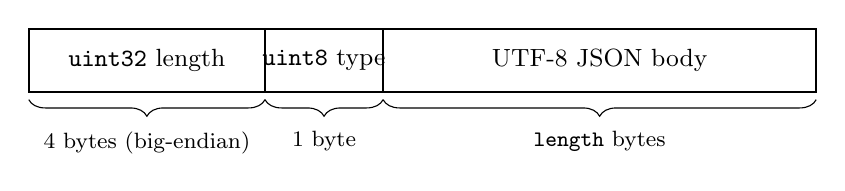
\begin{tikzpicture}[font=\small]
  \draw[thick] (0,0) rectangle (3, 0.8);
  \draw[thick] (3,0) rectangle (4.5, 0.8);
  \draw[thick] (4.5,0) rectangle (10, 0.8);

  \node at (1.5, 0.4) {\texttt{uint32} length};
  \node at (3.75, 0.4) {\texttt{uint8} type};
  \node at (7.25, 0.4) {UTF-8 JSON body};

  \draw[decorate, decoration={brace, amplitude=6pt, mirror}]
    (0, -0.1) -- (3, -0.1)
    node[midway, below=8pt, font=\footnotesize] {4 bytes (big-endian)};
  \draw[decorate, decoration={brace, amplitude=6pt, mirror}]
    (3, -0.1) -- (4.5, -0.1)
    node[midway, below=8pt, font=\footnotesize] {1 byte};
  \draw[decorate, decoration={brace, amplitude=6pt, mirror}]
    (4.5, -0.1) -- (10, -0.1)
    node[midway, below=8pt, font=\footnotesize] {\texttt{length} bytes};
\end{tikzpicture}
\end{center}
\begin{itemize}[leftmargin=1.5em]
  \item \textbf{length} (\texttt{uint32BE}): byte length of the JSON body only.
        The 5-byte header is not included in this count.
  \item \textbf{type} (\texttt{uint8}): message type identifier
        (from \texttt{GossipMessageType} or \texttt{ClientMessageType}).
  \item \textbf{body}: compact UTF-8 JSON.
\end{itemize}
\end{definition}

The total frame size is $5 + \mathit{length}$ bytes. The maximum permitted
body size is \texttt{limits.maxMessageBytes} (default: 10\,MiB).

\subsection{Message Type Constants}

\begin{table}[H]
\centering
\caption{Gossip and client protocol message type bytes.}
\label{tab:msg-types}
\begin{tabular}{@{}llll@{}}
\toprule
\multicolumn{2}{c}{\textbf{Gossip Protocol (port 7000)}} &
\multicolumn{2}{c}{\textbf{Client Protocol (port 7001)}} \\
\cmidrule(r){1-2}\cmidrule(l){3-4}
\textbf{Type} & \textbf{Byte} & \textbf{Type} & \textbf{Byte} \\
\midrule
\msg{HELLO}          & \texttt{0x01} & \msg{AUTH\_CHALLENGE}   & \texttt{0x10} \\
\msg{HELLO\_ACK}     & \texttt{0x02} & \msg{AUTH\_RESPONSE}    & \texttt{0x11} \\
\msg{HELLO\_CONFIRM} & \texttt{0x03} & \msg{AUTH\_ACK}         & \texttt{0x12} \\
\msg{PING}           & \texttt{0x04} & \msg{GET\_REQUEST}      & \texttt{0x20} \\
\msg{PONG}           & \texttt{0x05} & \msg{PUT\_REQUEST}      & \texttt{0x21} \\
\msg{DIGEST}         & \texttt{0x06} & \msg{DELETE\_REQUEST}   & \texttt{0x22} \\
\msg{REQUEST}        & \texttt{0x07} & \msg{KEYS\_REQUEST}     & \texttt{0x23} \\
\msg{MUTATIONS}      & \texttt{0x08} & \msg{ENTRIES\_REQUEST}  & \texttt{0x24} \\
\msg{ACK}            & \texttt{0x09} & \msg{GET\_RESPONSE}     & \texttt{0x30} \\
\msg{ERROR}          & \texttt{0x0a} & \msg{PUT\_RESPONSE}     & \texttt{0x31} \\
                     &               & \msg{DELETE\_RESPONSE}  & \texttt{0x32} \\
                     &               & \msg{KEYS\_RESPONSE}    & \texttt{0x33} \\
                     &               & \msg{ENTRIES\_RESPONSE} & \texttt{0x34} \\
                     &               & \msg{ERROR}             & \texttt{0x09} \\
\bottomrule
\end{tabular}
\end{table}

\subsection{Stream Decoder}

TCP is a byte-stream transport; a single \texttt{data} event may carry part of
a frame, a complete frame, or multiple frames. The \texttt{FrameDecoder} class
in \pkg{wire} maintains a reassembly buffer and emits complete frames:

\begin{enumerate}[leftmargin=1.5em]
  \item Incoming chunks are appended to an internal \texttt{Buffer}.
  \item The decoder checks whether the buffer contains at least 5 bytes (the
        header).
  \item If yes, it reads \texttt{length} from bytes 0--3 and \texttt{type}
        from byte 4.
  \item If \texttt{length} bytes of body are available (i.e., buffer length
        $\geq 5 + \mathit{length}$), the frame is extracted and emitted.
  \item If \texttt{length} exceeds \texttt{maxMessageBytes}, an error is emitted
        and the connection is closed, preventing OOM from a malformed or
        malicious message.
  \item The consumed bytes are removed from the buffer; the process repeats
        for any remaining data.
\end{enumerate}

This stateful push-based decoder correctly handles all TCP segmentation
scenarios and is tested with single-byte push streams.

\subsection{Encoding}

Frame encoding is straightforward:

\begin{lstlisting}[caption={Frame encoder (TypeScript).}]
export function encodeFrame(type: number, payload: unknown): Buffer {
  const body = Buffer.from(JSON.stringify(payload), "utf8");
  const frame = Buffer.allocUnsafe(5 + body.byteLength);
  frame.writeUInt32BE(body.byteLength, 0);
  frame.writeUInt8(type, 4);
  body.copy(frame, 5);
  return frame;
}
\end{lstlisting}

\subsection{DoS Considerations}

The \texttt{maxMessageBytes} limit defends against memory exhaustion by a peer
sending an oversized message. A frame with a \texttt{length} field exceeding
this limit triggers an immediate connection close without attempting to buffer
the body. This is the primary DoS surface in the current protocol; future
versions may add per-connection rate limiting and total in-flight byte limits.

% =============================================================================
% Section 11 — Persistence & Crash Recovery
% =============================================================================
\section{Persistence and Crash Recovery}
\label{sec:persistence}

Every \pebble{} node persists its state to an isolated data directory
(\texttt{dataDir}). The persistence layer ensures that no acknowledged
mutation is lost across node restarts and that the node can reconstruct its
full in-memory state on startup.

\subsection{On-Disk Layout}

\begin{lstlisting}[caption={Data directory layout.}, language={}]
dataDir/
  identity.json          # Node keypair and nodeId (generated once)
  metadata.json          # Atomic sequence and vector counter
  mutations.log          # Append-only NDJSON mutation log (with fsync)
  snapshots/
    2026-08-20T00-00-00-000Z.snapshot.json
    2026-08-21T00-00-00-000Z.snapshot.json
    ...
\end{lstlisting}

\subsection{Append-Only Mutation Log}

The \texttt{MutationLog} (\texttt{packages/core/src/persistence/log.ts})
appends each accepted local mutation to \texttt{mutations.log} as a single
newline-delimited JSON record (NDJSON format). Each append is followed by an
\texttt{fsync} call to flush the kernel buffer to durable storage before the
mutation is acknowledged to the caller.

\begin{definition}[Durability guarantee]
A mutation $m$ is \emph{durable} at node $n$ if $m$ has been serialised to
\texttt{mutations.log} and the \texttt{fsync} call has returned. Durable
mutations survive process crashes, OS crashes, and power failures (assuming the
storage medium respects \texttt{fsync} semantics).
\end{definition}

\begin{remark}[Gossip-received mutations]
Mutations received via gossip from peer nodes are applied to the in-memory store
and emitted as \texttt{mutation:applied} events. The orchestrator (\texttt{Pebble}
class) listens for these events and appends received mutations to the log as
well, ensuring that any mutation in the in-memory state is also represented
on disk.
\end{remark}

\subsection{Snapshots}

Taking a snapshot serialises the entire current state (including tombstones)
and the current version vector to a JSON file in \texttt{snapshots/}:

\begin{definition}[Snapshot]
A \emph{snapshot} $\mathcal{S}$ is a tuple
\[
  \mathcal{S} = \langle \mathit{version},\; t_\mathcal{S},\; V,\;
                        \mathit{nextSeq},\; S \rangle
\]
where $V$ is the version vector at snapshot time, $\mathit{nextSeq}$ is the
next local sequence number, and $S$ is the current state map
(key $\to$ winning mutation, including tombstones).
\end{definition}

Snapshot filenames are ISO 8601 timestamps safe for all operating systems
(colons replaced with hyphens). Lexicographic sort of filenames corresponds to
chronological order, enabling simple latest-snapshot selection.

Snapshots serve two purposes:
\begin{enumerate}[leftmargin=1.5em]
  \item \textbf{Faster recovery}: recovery needs only to replay log entries
        after the snapshot timestamp, rather than the full history.
  \item \textbf{Log truncation (future)}: once a snapshot is taken, older log
        entries that predate the snapshot can safely be discarded (\cref{sec:future}).
\end{enumerate}

\subsection{Crash Recovery Pipeline}

On node startup, the \texttt{recover} function reconstructs in-memory state
from the on-disk data:

\begin{algorithm}[H]
\caption{Node crash recovery (\texttt{recover})}
\label{alg:recovery}
\begin{algorithmic}[1]
\Require Node \texttt{dataDir}, empty \texttt{store}, \texttt{nodeId}
\State $\mathcal{S} \leftarrow \texttt{loadLatestSnapshot(dataDir)}$
\State $\mathcal{M} \leftarrow \texttt{loadMetadata(dataDir)}$
\State $\mathit{nextSeq} \leftarrow \mathcal{M}.\mathit{nextLocalSequence}$

\If{$\mathcal{S} \neq \bot$}
  \State $\texttt{store.importSnapshot}(\mathcal{S}.S,\; \mathcal{S}.V,\; \mathcal{S}.\mathit{nextSeq})$
  \State $\mathit{nextSeq} \leftarrow \max(\mathit{nextSeq},\; \mathcal{S}.\mathit{nextSeq})$
\Else
  \State $\texttt{store.setNextLocalSequence}(\mathit{nextSeq})$
\EndIf

\State $\mathit{log} \leftarrow \texttt{MutationLog(dataDir).readAll()}$
\For{each mutation $m$ in $\mathit{log}$}
  \State $\texttt{store.applyMutation}(m,\; \{\mathit{skipSignatureVerification}: \top\})$
  \If{$m.\mnid = \mathit{nodeId}$}
    \State $\mathit{nextSeq} \leftarrow \max(\mathit{nextSeq},\; m.\mseq + 1)$
  \EndIf
\EndFor

\State $\texttt{store.setNextLocalSequence}(\mathit{nextSeq})$
\end{algorithmic}
\end{algorithm}

\paragraph{Correctness argument.}
The log replay is idempotent: duplicate mutations (e.g., those already covered
by the snapshot) are silently skipped by the store's duplicate detection.
Mutations that arrived after the snapshot timestamp but before the crash are
replayed in full. The $\mathit{nextSeq}$ watermark is advanced to be strictly
greater than any local sequence seen, preventing sequence number reuse across
restarts (Invariant~\ref{inv:mono-seq}).

\subsection{Corrupted Log Tail}

If the node crashed mid-write, the last line of \texttt{mutations.log} may be
a truncated, invalid JSON record. The log reader handles this by discarding any
trailing partial line (lines that do not parse as valid mutations are skipped
with a warning). Since the line was not yet synced (the process crashed before
\texttt{fsync} returned), it was never acknowledged, and discarding it
preserves the durability guarantee.

% =============================================================================
% Section 12 — Complexity Analysis
% =============================================================================
\section{Complexity Analysis}
\label{sec:complexity}

This section analyses the computational and communication complexity of
\pebble{} as a function of the cluster size $N$ (number of nodes), the total
number of distinct keys $K$, and the total number of mutations $M$ in the
cluster history.

\subsection{Per-Node State Complexity}

\begin{table}[H]
\centering
\caption{In-memory state sizes per node.}
\label{tab:state-complexity}
\begin{tabular}{@{}lll@{}}
\toprule
\textbf{Structure} & \textbf{Size} & \textbf{Notes} \\
\midrule
Current state map ($S$)    & $\Oof{K}$   & One winning mutation per key,
                                            including tombstones \\
Mutation history ($H$)     & $\Oof{M}$   & All mutations ever received;
                                            no GC in v0.1 \\
Version vector ($V$)       & $\Oof{N}$   & One entry per known node \\
\bottomrule
\end{tabular}
\end{table}

The total in-memory footprint per node is $\Oof{K + M + N}$. In practice
$M \gg K$ after steady-state operation (many mutations per key), so the
dominant term is $\Oof{M}$.

\begin{remark}[History growth]
Because \pebble{} v0.1 retains the full mutation history without compaction,
memory usage grows without bound as long as mutations are generated. This is
the primary scalability concern in the current version; see
\cref{sec:limitations} and \cref{sec:future} for the planned GC mechanism.
\end{remark}

\subsection{Version Vector and Missing-Range Computation}

\begin{proposition}
Computing $\mathrm{missing}(V_A, V_B)$ requires $\Oof{N}$ time and produces
at most $N$ range entries.
\end{proposition}

\begin{proof}
The computation iterates over $\mathrm{dom}(V_A)$, which has at most $N$
entries (one per node). For each entry, a constant-time comparison and
conditional append are performed. The result has at most $N$ elements
(one per originating node). \qed
\end{proof}

\subsection{Gossip Round Complexity}

\begin{table}[H]
\centering
\caption{Per-gossip-round message complexity.}
\label{tab:round-complexity}
\begin{tabular}{@{}lll@{}}
\toprule
\textbf{Phase} & \textbf{Messages} & \textbf{Max Payload} \\
\midrule
DIGEST exchange      & 2 messages & $\Oof{N}$ bytes each \\
REQUEST (initiator)  & 1 message  & $\Oof{N}$ ranges \\
MUTATIONS (from B)   & 1 message  & $\Oof{M_{\max}}$ mutations \\
REQUEST (responder)  & 1 message  & $\Oof{N}$ ranges \\
MUTATIONS (from A)   & 1 message  & $\Oof{M_{\max}}$ mutations \\
ACK $\times 2$       & 2 messages & $\Oof{1}$ each \\
\midrule
\textbf{Total}       & \textbf{8 messages} &
  $\Oof{N + M_{\max}}$ bytes \\
\bottomrule
\end{tabular}
\end{table}

where $M_{\max} = \texttt{limits.maxMutationsPerMessage}$ (default: 500).

\paragraph{Worst-case bandwidth.}
If a node is starting fresh with no history and connects to a node with $M$
total mutations, it will require $\lceil M / M_{\max} \rceil$ gossip rounds to
catch up, each transferring $\Oof{M_{\max}}$ mutations. Total catch-up bandwidth:
$\Oof{M}$.

\paragraph{Incremental (steady-state) bandwidth.}
During steady-state operation with $\Delta M$ new mutations since the last sync
with a given peer, a single gossip round transfers $\Oof{\Delta M}$ mutations.
This is the common case.

\subsection{Cluster-Wide Convergence Time}

\pebble{} uses random gossip fanout of 1 per node per interval. This is
equivalent to the \emph{push-pull} gossip model studied by Demers et
al.~\cite{demers1987epidemic}.

\begin{theorem}[Expected convergence time]
\label{thm:convergence-time}
Starting from a single node holding a mutation, the expected number of gossip
rounds for the mutation to reach all $N$ nodes is $\Theta(N \log N)$, assuming
each node selects a uniformly random healthy peer in each round.
\end{theorem}

\begin{proof}[Sketch]
This follows from the standard coupon-collector analysis of epidemic
broadcasting. In round $r$, let $k$ be the number of informed nodes. Each of
the $N - k$ uninformed nodes is contacted by an informed node with probability
$k/N$ per round. By linearity of expectation and the harmonic series, the
expected total rounds until all nodes are informed is:
\[
  \mathbb{E}[\text{rounds}] = N \sum_{k=1}^{N} \frac{1}{k} = \Theta(N \log N).
\]
\qed
\end{proof}

\begin{table}[H]
\centering
\caption{Expected convergence rounds for representative cluster sizes
with \texttt{gossipIntervalMs} = 1{,}000\,ms.}
\label{tab:convergence-table}
\begin{tabular}{@{}rrrr@{}}
\toprule
$N$ & $\mathbb{E}[\text{rounds}]$ & \textbf{Approx.\ wall time} & \textbf{Note} \\
\midrule
3   & $\approx 5.5$ & $\approx 5.5\,\text{s}$  & Small dev cluster \\
5   & $\approx 11$  & $\approx 11\,\text{s}$   & Small production \\
10  & $\approx 29$  & $\approx 29\,\text{s}$   & Medium cluster \\
20  & $\approx 72$  & $\approx 72\,\text{s}$   & Large cluster \\
50  & $\approx 225$ & $\approx 225\,\text{s}$  & Use higher fanout \\
100 & $\approx 519$ & $\approx 519\,\text{s}$  & Use higher fanout \\
\bottomrule
\end{tabular}
\end{table}

\begin{remark}[Fanout scaling]
For clusters larger than $\sim$20 nodes, a gossip fanout greater than 1
(selecting $f > 1$ peers per round) reduces convergence time to
$\Theta(\log N / \log f)$ rounds. This is a planned improvement
(\cref{sec:future}).
\end{remark}

\subsection{Gossip Session Load per Node}

Each node initiates exactly one outbound gossip session per
\texttt{gossipIntervalMs} interval and can receive an unbounded number of
inbound sessions (one per active peer). In a cluster of $N$ nodes:

\begin{itemize}[leftmargin=1.5em]
  \item \textbf{Outbound load}: $\Oof{1}$ session per node per interval (constant).
  \item \textbf{Inbound load}: $\Oof{N}$ sessions per interval, since every
        other node may choose this node as its target.
\end{itemize}

Each inbound session occupies a dedicated TCP connection for the duration of
the 4-step protocol. Because gossip sessions are short-lived and sequential per
initiator, the server must handle up to $N-1$ concurrent inbound connections.
The Node.js event loop can sustain hundreds of concurrent lightweight connections
without saturation.

\subsection{Handshake Complexity}

The 3-way handshake (\cref{sec:nodeauth}) requires 3 round trips and 4
Ed25519 operations (2 signs, 2 verifies) per connection. All operations are
$\Oof{1}$ in node count and dominate only the connection-establishment phase.

\subsection{Snapshot and Recovery Complexity}

\begin{table}[H]
\centering
\caption{Persistence operation complexity.}
\label{tab:persistence-complexity}
\begin{tabular}{@{}ll@{}}
\toprule
\textbf{Operation} & \textbf{Complexity} \\
\midrule
Snapshot write     & $\Oof{K}$ — serialise current state (one entry per key) \\
Snapshot read      & $\Oof{K}$ — deserialise and validate \\
Log append         & $\Oof{1}$ amortised — single NDJSON line + fsync \\
Log replay         & $\Oof{M}$ — replay all entries (bounded by $M$) \\
Recovery (total)   & $\Oof{K + M}$ — snapshot load + log replay \\
\bottomrule
\end{tabular}
\end{table}

% =============================================================================
% Section 13 — System Invariants
% =============================================================================
\section{System Invariants}
\label{sec:invariants}

\pebble{} maintains eight core invariants across all subsystems. These
invariants collectively guarantee correctness, security, and eventual
consistency.

\begin{invariant}[Global Uniqueness]
\label{inv:uniqueness}
The pair $(\mnid, \mseq)$ uniquely identifies at most one mutation across the
entire cluster:
\[
  \forall m, m' \in \MutSet:\quad
  m.\mnid = m'.\mnid \;\land\; m.\mseq = m'.\mseq
  \;\implies\; m = m'.
\]
\textit{Enforcement:} The Store's \texttt{applyMutation} checks whether $\mathrm{id}(m)$
is already in the history map $H$. If it is and the content differs, a
\texttt{SequenceCollisionError} is thrown and the mutation is rejected. Only
exact duplicates (same content) are silently accepted as idempotent.
\end{invariant}

\begin{invariant}[Immutability]
\label{inv:immutability}
Once a mutation $m$ is stored in $H$, its fields are never modified.
\[
  \forall t, t' > 0:\; m \in H^t \;\implies\; H^{t'}[\mathrm{id}(m)] = m.
\]
\textit{Enforcement:} All mutation fields are declared \texttt{readonly} in
TypeScript. The in-memory map stores references to frozen objects; no code path
modifies a mutation after creation.
\end{invariant}

\begin{invariant}[Authenticity]
\label{inv:authenticity}
Every mutation stored in $H$ that originated from a remote peer carries a valid
Ed25519 signature from the node identified by $m.\mnid$:
\[
  \forall m \in H_{\mathrm{remote}}:\;
  \mathrm{Ed25519Verify}(pk_{m.\mnid},\;
  \mathrm{canonicalEncode}(m_{\text{sign}}),\; m.\msig) = \top.
\]
\textit{Enforcement:} \texttt{applyMutation} with
\texttt{skipSignatureVerification~=~false} (the default for all network paths)
performs verification before committing. An invalid signature raises
\texttt{InvalidSignatureError}.
\end{invariant}

\begin{invariant}[Idempotence]
\label{inv:idempotence}
Applying the same mutation $m$ to a store multiple times produces the same
result as applying it once:
\[
  \forall m:\; \texttt{apply}(\texttt{apply}(S, m), m) = \texttt{apply}(S, m).
\]
\textit{Enforcement:} If $\mathrm{id}(m) \in H$, \texttt{applyMutation}
returns immediately without touching state. Gossip may deliver the same
mutation multiple times (e.g., via two independent peers); idempotence ensures
no harm.
\end{invariant}

\begin{invariant}[Deterministic Ordering]
\label{inv:det-order}
Given the same set of mutations $M$ for a key $k$, every node independently
computes the same winning mutation:
\[
  \forall n_1, n_2:\;
  H_{n_1} \cap \{m : m.\mkey = k\} = H_{n_2} \cap \{m : m.\mkey = k\}
  \;\implies\; S_{n_1}(k) = S_{n_2}(k).
\]
\textit{Enforcement:} The LWW \texttt{compare} function is a pure function of
the mutation's fields. It uses no node-local state, no random values, and no
external communication. By \cref{thm:convergence}, this implies convergence.
\end{invariant}

\begin{invariant}[Tombstone Replication]
\label{inv:tombstone}
If a \texttt{delete} mutation $m_d$ for key $k$ exists in the cluster, it is
eventually present in every node's history $H$ and wins over any prior
\texttt{put} mutation:
\[
  \exists n:\; m_d \in H_n \;\implies\;
  \forall n':\; \text{eventually}\; m_d \in H_{n'}.
\]
\textit{Enforcement:} Tombstones are stored in $H$ and replicated through gossip
exactly like put mutations. The LWW order ensures a tombstone with a higher
timestamp wins over prior puts (absent concurrent puts with a higher timestamp).
\end{invariant}

\begin{invariant}[Monotonic Version Vectors]
\label{inv:mono-vec}
Version vector entries are non-decreasing over time:
\[
  \forall n, n':\; V_n^t[n'] \leq V_n^{t+\epsilon}[n'].
\]
\textit{Enforcement:} The \texttt{advanceVector} function uses
$V[n] \leftarrow \max(V[n], m.\mseq)$. No code path decreases a vector entry.
Proved in Invariant~\ref{inv:mono-vv}.
\end{invariant}

\begin{invariant}[Monotonic Sequences]
\label{inv:mono-seq}
The local sequence counter at a node never repeats or regresses across restarts:
\[
  \forall t, t' > 0,\; t < t':\; \mathit{nextSeq}^t_n \leq \mathit{nextSeq}^{t'}_n.
\]
\textit{Enforcement:} The crash recovery algorithm (\cref{alg:recovery}) sets
$\mathit{nextSeq}$ to the maximum of the metadata value, the snapshot value,
and one more than the highest local sequence seen in the log. A node starting
with an empty log and metadata initialises $\mathit{nextSeq} = 1$.
\end{invariant}

% =============================================================================
% Section 14 — Known Limitations
% =============================================================================
\section{Known Limitations (v0.1)}
\label{sec:limitations}

The current version of \pebble{} makes several deliberate simplifications that
limit its applicability in certain scenarios. This section catalogues each
limitation honestly, explains why it exists, and references the corresponding
future-work item.

\subsection{Physical Wall-Clock Timestamps}

\textbf{Impact:} The LWW total order uses $m.\mts$ as the primary comparison
key (\cref{def:lww-order}). Nodes with skewed clocks can produce mutations that
lose to older writes from well-clocked nodes, even when the skewed node's write
is causally later.

\textbf{Example:} Node $A$'s clock is 5\,s behind. Node $B$ writes $k = v_1$ at
$t = 1000$. Node $A$ writes $k = v_2$ at $t = 997$ (real time 1002). Despite
$A$'s write being causally later, $v_1$ wins because $1000 > 997$.

\textbf{Severity:} Low in practice for clusters with NTP-synchronised clocks
(typical drift $< 100\,\text{ms}$), but potentially problematic in WAN deployments
or environments with unreliable time sources.

\textbf{Planned fix:} Hybrid Logical Clocks~\cite{kulkarni2014hlc} (\cref{sec:future}).

\subsection{Contiguous-Sequence Assumption in Version Vectors}

\textbf{Impact:} \pebble{}'s version vector records only the highest sequence
seen from each node, implying that all lower sequences have been received.
This assumption holds only when mutations arrive in order within a single TCP
connection. If future versions add parallel or unreliable delivery, the
high-water mark can skip over missing mutations.

\textbf{Severity:} Currently safe, because all gossip delivery occurs over a
single ordered TCP stream per session. Not safe if multi-path delivery or
UDP-based gossip is introduced without a corresponding change to the vector
representation.

\textbf{Planned fix:} Sparse version vectors using bitmap or interval-tree
representation (\cref{sec:future}).

\subsection{Unbounded History Growth}

\textbf{Impact:} The mutation history $H$ retains every mutation ever seen.
Memory usage grows linearly with total mutation count $M$ with no bound.
On-disk log size also grows unboundedly.

\textbf{Severity:} High for long-running deployments with high write throughput.
A node writing 1,000 mutations/second accumulates $\sim$86 million mutations
per day, each consuming roughly 200 bytes, resulting in $\sim$17\,GB/day.

\textbf{Planned fix:} Snapshot-based GC that discards log entries and history
entries for mutations older than the latest snapshot, retaining only
the winning mutation per key (\cref{sec:future}).

\subsection{No Multi-Key Atomicity}

\textbf{Impact:} \pebble{} does not support multi-key transactions. A client
performing a sequence of puts over a key group has no guarantee that an
intermediate state (some keys updated, others not) is invisible to concurrent
readers.

\textbf{Severity:} Applications requiring atomic updates to multiple keys (e.g.,
transferring a value from key $A$ to key $B$) cannot be implemented correctly
with \pebble{} v0.1.

\textbf{Planned fix:} Optimistic concurrency control or saga patterns
(\cref{sec:future}).

\subsection{Static Cluster Membership}

\textbf{Impact:} The set of nodes is defined at startup via \texttt{cluster.json}.
Adding or removing a node requires updating the configuration file and
restarting all nodes to reload it. There is no online join/leave mechanism.

\textbf{Severity:} Moderate. Affects operational flexibility but not correctness;
the cluster continues to function with the existing node set.

\textbf{Planned fix:} A CRDT-based membership view with Paxos-free join/leave
propagation (\cref{sec:future}).

\subsection{Gossip Fanout Fixed at 1}

\textbf{Impact:} Each node initiates exactly one gossip session per interval.
Convergence time grows as $\Theta(N \log N)$ (\cref{thm:convergence-time}),
which becomes impractically slow for large clusters ($N > 50$).

\textbf{Severity:} Low for small clusters; significant for large ones.

\textbf{Planned fix:} Configurable fanout $f > 1$, reducing convergence to
$\Theta(\log N / \log f)$ rounds.

\subsection{No Transport-Layer Encryption}

\textbf{Impact:} Gossip and client traffic is transmitted as plaintext JSON over
raw TCP. An on-path adversary can read mutation contents and client credentials
in transit.

\textbf{Severity:} High in untrusted network environments. The Ed25519
authentication layer prevents \emph{impersonation} and \emph{mutation
injection}, but not \emph{eavesdropping}.

\textbf{Planned fix:} TLS for both the gossip and client ports (\cref{sec:future}).

% =============================================================================
% Section 15 — Future Work
% =============================================================================
\section{Future Work}
\label{sec:future}

This section outlines the planned evolution of \pebble{} beyond v0.1, grouped
by impact and estimated implementation complexity.

\subsection{Hybrid Logical Clocks (HLC)}

\textbf{Motivation:} Replace physical wall-clock timestamps with Hybrid Logical
Clocks~\cite{kulkarni2014hlc} to capture causality between events, even under
clock skew.

\textbf{Approach:} Each node maintains an HLC state $(l, c)$ where $l$ is the
maximum of the local physical clock and the highest $l$ seen in received
messages, and $c$ is a counter that breaks ties at the same $l$ value. The HLC
advances monotonically and satisfies $l \geq \mathrm{now}()$ at all times,
ensuring that causally later events always receive larger HLC values.

\textbf{Impact:} The LWW comparison function (\cref{def:lww-order}) would
replace $m.\mts$ with the HLC value, eliminating clock-skew-induced inversions.
The mutation wire format would add an HLC component alongside the physical
timestamp. Backward compatibility requires a protocol version bump.

\subsection{Sparse Version Vectors}

\textbf{Motivation:} Remove the contiguous-sequence assumption to support
out-of-order mutation delivery and multi-path replication.

\textbf{Approach:} Replace the high-water mark integer $V[n]$ with a compact
set representation of received sequence numbers (e.g., a sorted interval list
or a roaring bitmap~\cite{riak2010}). The \texttt{getMissingRanges} function
would compute gaps in the received set rather than the single suffix above the
watermark.

\textbf{Impact:} Memory overhead per node increases by a constant factor. Gossip
requests become slightly larger (a list of gaps rather than a single range).
Enables future UDP-based or multi-path gossip without correctness risk.

\subsection{History Compaction and Tombstone GC}

\textbf{Motivation:} Bound memory and on-disk storage by discarding history
entries for mutations that are no longer needed for gossip sync.

\textbf{Approach:} Periodically take a snapshot and promote it to a
\emph{stable checkpoint}. All history entries for mutations covered by the
checkpoint can be discarded. Gossip peers that have not yet received those
mutations must be directed to fetch the snapshot instead of individual mutations
(a form of state transfer).

Tombstone GC requires additional coordination: a tombstone can only be discarded
if all nodes in the cluster have seen it. A simple mechanism is a cluster-wide
minimum version vector: $V_{\min}[n] = \min_{i} V_i[n]$ over all nodes. History
entries with sequence $\leq V_{\min}[n]$ are safe to discard.

\textbf{Impact:} Bounds $|H|$ to $\Oof{K}$ after compaction (one entry per key).
Requires nodes that fall far behind to perform a full state transfer rather than
incremental gossip.

\subsection{Dynamic Cluster Membership}

\textbf{Motivation:} Allow nodes to join or leave the cluster without restarting
all nodes or manually editing \texttt{cluster.json}.

\textbf{Approach:} Represent the cluster membership as a CRDT (e.g., a 2P-Set
or OR-Set) replicated through the gossip protocol. A joining node broadcasts a
signed join request; existing nodes add it to the membership CRDT and begin
gossiping with it. A leaving node broadcasts a signed leave message. The
moderator signs membership changes to prevent rogue nodes from injecting
themselves.

\textbf{Impact:} Eliminates the need for out-of-band cluster reconfiguration.
Requires all nodes to run a compatible membership CRDT implementation.

\subsection{Multi-Key Transactions}

\textbf{Motivation:} Provide atomic read-modify-write and multi-key update
semantics for applications that require them.

\textbf{Approach:} Two candidate approaches:
\begin{enumerate}[leftmargin=1.5em]
  \item \textbf{Optimistic concurrency control (OCC):} The client reads a set
        of keys with their current version vectors, applies changes, and submits
        a conditional write that is rejected if any observed version has changed.
        Conflicts are retried by the client.
  \item \textbf{Saga pattern:} Multi-key updates are composed as a sequence of
        compensating single-key mutations. Partial failures leave a detectable
        intermediate state that can be rolled back.
\end{enumerate}
Full distributed serialisable transactions would require a consensus layer
(contradicting the leaderless design goal) and are not planned.

\subsection{TLS Transport Encryption}

\textbf{Motivation:} Protect mutation contents and client credentials from
on-path eavesdroppers.

\textbf{Approach:} Wrap both the gossip port and the client port in TLS 1.3.
Peer authentication during the TLS handshake can reuse the existing Ed25519
keys, eliminating the need for a separate PKI (mTLS with self-signed certs
derived from the Ed25519 identity). The application-level handshake
(\cref{sec:nodeauth}) could be simplified or merged with the TLS handshake.

\subsection{Configurable Gossip Fanout}

\textbf{Motivation:} Reduce convergence time for large clusters by initiating
$f > 1$ gossip sessions per interval.

\textbf{Approach:} Expose a \texttt{gossipFanout} parameter in
\texttt{cluster.json}. The \texttt{GossipEngine} selects $f$ random healthy
peers per interval and runs sessions concurrently. Expected convergence time
drops to $\Theta(\log_f N)$ rounds, as each round covers an $f$-fold more ground.

\subsection{Read Repair and Anti-Entropy}

\textbf{Motivation:} Detect and repair state divergence that persists beyond
the normal gossip window (e.g., due to prolonged partitions or log corruption
on a specific node).

\textbf{Approach:} A periodic anti-entropy pass computes a Merkle tree over
the current state and compares digests with all peers. Divergent subtrees are
repaired by re-exchanging the affected mutations. This provides a background
consistency guarantee independent of the gossip fanout.

\subsection{Read Consistency Modes}

\textbf{Motivation:} Offer stronger read guarantees for applications that need
them, without abandoning the leaderless design for writes.

\textbf{Approach:} Two optional read modes:
\begin{description}[leftmargin=1.5em]
  \item[Read-your-writes:] After a write at node $n$, route subsequent reads
        for the same key to $n$ until the version has propagated.
  \item[Monotonic reads:] Track a client-side version vector; reject reads from
        nodes whose vector does not dominate the client's last-observed vector.
\end{description}
Both modes are implementable without consensus and add only client-side
bookkeeping overhead.

% =============================================================================
% Section 16 — Conclusion
% =============================================================================
\section{Conclusion}
\label{sec:conclusion}

This whitepaper has presented \pebble{}---a leaderless, eventually consistent,
distributed key-value store built on a small set of composable primitives.

The system's correctness rests on three interlocking formal foundations.
First, the LWW total order (\cref{def:lww-order}, \cref{thm:total-order})
ensures that any set of mutations for a key has a unique maximum element,
and that every node in possession of the same set independently computes the
same winner (\cref{thm:convergence}). Second, version vectors provide a
compact summary of each node's history state, enabling the gossip protocol
to compute precisely which mutations a peer is missing in $\Oof{N}$ time
(\cref{sec:vv}). Third, Ed25519 signatures bound to canonical JSON encodings
ensure that only authorised nodes can produce valid mutations and only
moderator-credentialed clients can access the store (\cref{sec:crypto}).

The 4-step symmetric gossip protocol (\cref{sec:gossip}) is deadlock-free,
idempotent, and bandwidth-efficient: in steady state it transfers only the
$\Delta M$ mutations since the last sync with a given peer. The expected
cluster-wide convergence time is $\Theta(N \log N)$ rounds for fanout-1 gossip,
converging to a few minutes for practical small-to-medium clusters
(\cref{tab:convergence-table}).

The eight core invariants (\cref{sec:invariants}) are enforced structurally
by the implementation: global uniqueness by sequence collision detection,
immutability by TypeScript readonly types, authenticity by mandatory signature
verification on all network paths, and monotonicity by the $\max$-based vector
advancement rule.

\pebble{} is intentionally minimal in v0.1: no leader election, no consensus,
no dynamic membership, no transport encryption. These choices make the system
easy to reason about, easy to deploy, and easy to extend. The limitations
documented in \cref{sec:limitations} and the roadmap in \cref{sec:future}
chart a clear path toward a more capable system that preserves the leaderless,
eventually consistent design philosophy.

\paragraph{Implementation status.}
\pebble{} is implemented in TypeScript on Node.js, structured as a pnpm
monorepo of seven packages. The test suite comprises 121 automated tests
covering unit logic, failure modes, and end-to-end multi-node scenarios
including 3-node convergence, network partition healing, crash recovery,
security rejection of forged mutations, and randomised chaos testing across
hundreds of concurrent writes.

\paragraph{Availability.}
The source code is available at
\url{https://github.com/neon-x-hub/pebble} under the MIT licence.


% ---------------------------------------------------------------------------
% Bibliography
% ---------------------------------------------------------------------------
\newpage
\bibliographystyle{abbrv}
\bibliography{references}

\end{document}
